\chapter{Introducing Power Compensations}
\label{cha:power_compensations}

\minitoc

\section{Introduction}

In this chapter, we propose some heuristics to solve the problem from the model presented in Section \ref{sec:ODM}. The main objective is to adapt the offline plan according to real power production and usage. First, we describe the heuristics to solve it, linking with the model from Chapter \ref{cha:model}. Then, we explain the experimental environment used in the experiments. Finally, we present and discuss the results, highlighting the impact of the power constraints.

\section{Proposed Approach}

We divided the heuristic into two parts. First, we detail the scheduling decisions. The scheduler defines the job priority and placement. Also, the scheduler tries to avoid killing jobs, demanding more power if needed. Then, we describe the power compensation heuristics. These heuristics approximate the battery's state of charge from the target level.

\subsection{Scheduling}
\label{sec:heuristic_scheduling}

Job scheduling is a well-known problem NP-complete problem \cite{robert2009introduction, agrawal2021energy}. Several heuristics are proposed to solve this problem in an acceptable time. We implemented a well-known algorithm named EASY Backfilling in this chapter \cite{mu2001utilization}. This heuristic is known for its simple and robust implementation \cite{srinivasan2002characterization}. Also, it maximizes server utilization \cite{srinivasan2002characterization}. This algorithm englobes queue sorting and placement. First, it places priority jobs in the available servers. Then, it fills the scheduling holes with small jobs (see Figure \ref{fig:backfilling}). Algorithm \ref{alg:algo_scheduling} denotes a pseudo-code of EASY Backfilling, presented by \citeauthor{lelong2018tuning} as EASY-$P_{R}$-$P_{B}$ policy \cite{lelong2018tuning}. ODM uses this heuristic when a job arrives, a job finishes or new servers are available. 

\IncMargin{1em}
\begin{algorithm}[!htb]
    \LinesNumbered
    \footnotesize
    \SetAlgoLined
    \SetKwInOut{Input}{input}\SetKwInOut{Output}{output}
    \Input{Queue $Q$ of waiting jobs, $P_{R}$ as priority order, and $P_{B}$ as backfilling order.}
    \Output{None (calls to \textit{Start()})}
    \Begin{
        Sort $Q$ according to $P_{R}$\;
        \For{job $j$ in $Q$}{
            Pop $j$ from $Q$\;
            $S_j \leftarrow$ \textit{select\_servers($j$)}\;
            \uIf{$j$ can be started in servers $S_j$}{
                \textit{Start($j$, $S_j$)}\;
            }\Else{
                Reserve $j$ at the earliest time possible according to the walltime of the currently running jobs\;
                Sort $Q$ according to $P_{B}$\;
                \For{job $j^{'}$ in $Q$}{
                    $S_j \leftarrow$ \textit{select\_servers($j^{'}$)}\;
                    \If{$j^{'}$ can be started in servers $S_j$ without delaying the reservation on $j$}{
                        \textit{Start($j^{'}$, $S_j$)}\;
                    }
                }
                \textbf{break}\;
            }
        }
    }
    \caption{EASY-$P_{R}$-$P_{B}$ scheduling \cite{lelong2018tuning}.}
    \label{alg:algo_scheduling}
\end{algorithm}
\DecMargin{1em}

First, this heuristic sorts the jobs in the queue in a priority order $P_{R}$ (line 2). Then, it selects the servers to run this job (line 5). If the job $j$ can start in the servers $S_j$ (line 6), it places the job in the servers (line 7). When it finds a job that can not be placed now, it starts to backfill (lines 9-17). Then, it reserves the first moment to run this job (named priority job) in the future (line 9). So, it re-sorts the queue using $P_{B}$ (line 10), placing the other jobs in the servers (lines 11-16) without delaying the (future) priority job execution (line 13). As presented, the algorithm sorts the queue using $P_{R}$ (in the priority moment) and $P_{B}$ (in the backfilling moment). However, the typical implementation uses the same sort for both \cite{lelong2018tuning}. Our first implementation uses the typical algorithm (same sorting policy), but Chapter \ref{cha:heuristic} uses two policies. Thus, $P_{R}$ and $P_{B}$ apply Descending Bounded Slowdown (higher Bounded Slowdown first) policy from Equation \ref{equ:slowdown}. This order helps to let a job wait proportionately to its size.

Besides the placement, the scheduler maintains the jobs running at least at a "minimal speed". This minimal speed is given by Equation \ref{equ:avoid_walltime}. The idea is to keep the jobs' servers at the speed $D_{s,d}$. For example, if $D_{s,d}$ is too slow, the job can reach the walltime without finishing all its computing. Also, if the offline plan indicates to sedate a server, the jobs running on this server are killed. So, every time step $t$, the scheduler verifies the energy needed to maintain the jobs running at least at the minimal speed. If it is necessary to use more energy now (changing the plan), it verifies if it is possible to migrate power from the future to now. This verification consists of two tests:
\begin{enumerate}
    % \item \textit{Does the battery have the energy to be migrated?} The algorithm calculates how much battery energy is planned to be used in the future. The algorithm must let minimal energy to maintain all servers in the sleep state (it can come from battery, renewable, or hydrogen). So, the energy needed to maintain jobs running must be present in the sum of future usage;
    % In this test, the algorithm verifies the battery usage in future steps. Let $P_{min}$ be the power needed to maintain all servers in the sleeping state. So, for each step, the energy possible to migrate from the batteries is equal to:
    % \begin{itemize}
        %     \item If $P_{fc} > P_{min}$: $P_{renew} + P_{dch} - P_{ch}$. In this case, hydrogen maintains the servers in the sleeping state. So all renewable can be used to charge the battery;
        %     \item If not: $P_{renew} + P_{dch} - P_{ch} - P_{ez} - P_{min}$
        % \end{itemize}
    \item \textit{Will battery boundaries be violated?} Equation \ref{equ:battery_boundaries} must be respected. So, migration can not violate the SoC boundaries;
    \item \textit{Is it possible to compensate for this change?} This verification is explained in Section \ref{sec:power_compensation};
\end{enumerate}

If possible, the scheduler modifies the offline IT plan to let the servers run at the speed $D_{s,d}$. If it is not possible, the scheduler does not change the offline plan. 

\subsection{Power compensations}
\label{sec:power_compensation}

After describing the scheduling algorithm, this section explains the heuristic to compensate for power fluctuations presented in Section \ref{sec:ODM}. The objective of power compensations is to ensure that $SoC$ and $LoH$ are close to the offline plan at the end of the time window. Therefore, every time step $t$, ODM calculates $E_{comp}$ using Equation \ref{equ:energy_battery}. $E_{comp}$ can be positive or negative, according to battery usage or renewable production. Thus, the problem is to define the future time step to change power usage to use the energy $E_{comp}$. Let $t'$ be the future time step. Then, ODM must change $P_{dch}(t')$ and $P_{ch}(t')$. Of course, $P_{dch}$ and $P_{ch}$ are power, and $E_{comp}$ is energy, so we make the conversion from power to energy in this process. Also, the changes must consider the boundaries from Equations \ref{equ:discharge_boundary} and \ref{equ:charge_boundary}. In addition, even if all servers are sleeping, minimal power must be delivered since the power usage in the sleep state is not zero. Let $P_{min}$ be the minimal power possible. Then, $P_{prod}(t') \ge P_{min}$, considering that $P_{prod}$ comes from Equation \ref{equ:model_energy}. Nevertheless, the compensation still considers the estimated renewable production from the future steps.

ODM spreads the energy over different $t'$ until all modifications compensate for $E_{comp}$. The power compensations happen in two cases:
\begin{enumerate}
    \item Every time step, ODM recalculates $SoC(T)$ using Equation \ref{equ:battery_energy} from the actual step until $T$. Then, it compares $SoC(T)$ and $SoC_{target}$, using Equation \ref{equ:delta_energy}. Finally, ODM compensates $E_{comp}$ (from Equation \ref{equ:energy_battery}), approximating $SoC(T)$ to $SoC_{target}$ (respecting Equation \ref{equ:soc_target});
    \item When the scheduler demands more power, as presented in Section \ref{sec:heuristic_scheduling}, it tries to maintain the servers with jobs running. So, it increases the power usage at the step. This increase will change the $SoC(T)$, demanding compensation. This compensation is always negative (if ODM uses more power now, it needs to use less in the future).
\end{enumerate}

If ODM can not entirely compensate $E_{comp}$, it has two possible actions. If the request for compensation comes from the scheduler (case 2), it does not make the modifications demanded by the scheduler, impacting the jobs. On the other hand, in case 1, ODM will modify as much as possible. On Datazero2, the impossibility of compensating for case 1 can start a new negotiation from the offline part to deal with this event. However, in this thesis we let the ODM run to see the impact of these cases.

The question now is: in which future time step $t'$? To answer this, we propose four policies: \emph{Peak}, \emph{Next}, \emph{Last}, and \emph{Load}. Figure \ref{fig:compensation} illustrates an example of these policies. The \emph{Next} and \emph{Last} policies execute the same search independently of the type of compensation (positive or negative compensation). While the \emph{Next} policy takes the $t + 1$, \emph{Last} policy takes $T$. On the other hand, \emph{Peak} and \emph{Load} take different steps according to the compensation (positive or negative). \emph{Peak} policy finds the higher power production ($P_{prod}$) peak in negative compensation and the lower peak in positive compensation. This policy will "shave" the peaks, tending to a flat curve. \emph{Load} policy considers the different between demand ($P_{load}$) and production ($P_{prod}$). In positive compensation, this policy takes the higher difference $P_{load} - P_{prod}$, while in negative it takes the smaller one. In Figure \ref{fig:compensation}, if the scheduler saves energy at step 1, it could compensate for it at step 3 (\emph{Next}), step 12 (\emph{Peak}), step 15 (\emph{Last}), or step 14 (\emph{Load}). Even if Figure \ref{fig:compensation} compensates only one time, the algorithm can select more than one until compensate $E_{comp}$ entirely and follows its policy (e.g., Next will take step 2, 3, 4, etc.).

\begin{figure}[!htb]
    \centering
    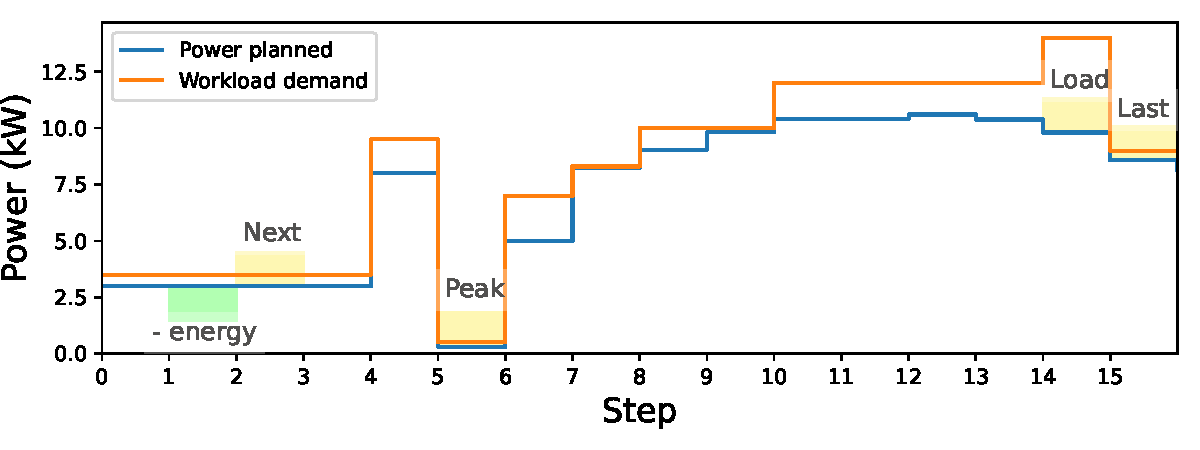
\includegraphics[scale=0.7]{Images/Compensations/policies.pdf}
    \caption{Compensation policies. The blue curve is the offline usage plan ($P_{prod}$) and the orange line is the estimated demand ($P_{load}$). In this example, it saves some energy in time step 1 (see the green square). So, it can reintroduce this energy in future time steps (see the yellow squares).}
    \label{fig:compensation}
\end{figure}

Finally, the last part of the heuristic is transforming the power modifications into server configuration. Since the IT offline plan gives the P-state of the servers for each step $t$, we must adapt this plan for the new power. We propose a heuristic to find quick solutions. The four policies use the same heuristic to distribute the compensation. This heuristic has a list of all power and speed differences between two P-states, so it can fastly decide which one will impact the most on data center speed. First, it calculates the difference between the power usage in the offline plan and the power to use. If this difference is positive, it can improve the server configuration, speeding up or turning on servers. It goes through the list searching for the highest flops improvement below or equal to the power increment. It does it in the following order:
\begin{enumerate}
    \item Find the highest improvement possible for the servers running some job;
    \item Find the highest improvement possible for the idle servers.
\end{enumerate}

Taking Table~\ref{tab:gros} as an example, let's say that we have two servers running jobs: one on state 5 and another on state 10. If the system has 30 W to increase, it will increase first the server on state 10 to state 1, because it will increase 14.41 Gflops (against 6.45 Gflops from state 5 to state 1). If a server is sleeping, it also considers the power needed to turn the server on. When the difference between offline and online power is negative, the algorithm must reduce the speed of the servers. So, it does the following:
\begin{enumerate}
    \item Reduce the speed of idle servers;
    \item Reduce the speed of the servers running jobs. We calculate $(wall_{j} - elapTime_{j})$ for each job. Then, we sort the servers by this value in decreasing order.
\end{enumerate}

It stops after the first modification which let the power usage lower or equal to the power production $P_{prod}(t)$. The second step will reduce servers' speed with more time to compensate for this reduction in the future. It is better to maintain jobs closer to finish with the maximum speed, granting that they will complete.

\section{Experimental environment}
\label{sec:experiment_environment}
% IT (servers)
% Electrical (battery, solar, wind, etc)
% Workload Trace
% Weather Trace

In this section, we present the environment used to run our simulations. This environment englobes IT servers definition, electrical elements, and the workload and weather traces. We focus on simulating a time window of three days ($T_{w}=259200 s$), divided into time steps of 5 minutes ($\Delta t=300$). We chose time steps of 5 minutes because it is neither too long to react to events nor too short for server transitions. For example, a time step of 1 minute is good for adapting the battery usage, but it is not enough to turn on a server (Table \ref{tab:gros} shows that a Gros server takes 164 seconds to finish the off$\rightarrow$on transition). A longer time step can be too late to adapt battery usage. Regarding the server specification, we simulated a homogeneous data center using the GRID5000's Gros server. Their parameters were presented in Table \ref{tab:gros}. We present the experiments in a homogeneous data center to ease the understanding. However, we present different experiments in a heterogeneous data center in \cite{de2022analyzing}. Our data center is composed of 400 servers with Gros specifications. Other aspects, such as network and memory are ignored. 

Considering the electrical components, the data center is composed of solar panels, wind turbines, batteries, and one hydrogen tank. The total size of the batteries is 800 kWh ($B_{size}=800kWh$). The efficiency of charging is 0.82 ($\eta_{ch}=0.82$) and discharging is 1.22 ($\eta_{dch}=1.22$). We defined the thresholds $SoC_{min}$ and $SoC_{max}$ as 20\% and 90\%. So, the range of available energy from the battery allows to run the whole data center for 9.76 hours. We set the max charge and discharge power as 80\% of the battery size ($P_{ch_{max}}=640kW$ and $P_{dch_{max}}=640kW$). The hydrogen tank has 20000 kg ($LoH_{max}=20000$), with the electrolyzer's efficiency of 97.5 and the fuel cell's efficiency of 13.332. We defined that the battery starts half charged ($SoC(0)=50\%$) and the hydrogen with 300 kg ($LoH(0)=300kg$). We defined also that they should come back at least to the same value as they started at the end of the time window ($SoC_{target} = 50\%$ and $LoH_{target}=300kg$).

Regarding workload and weather traces, we have divided the experiments into two parts. The first part aims to analyze the decisions in critical scenarios (named \emph{critical scenarios}) and the second part focuses on the average cases (named \emph{average scenarios}). 

\subsection{Critical Scenarios}

In the first part, we have taken two workloads from the Metracentrum dataset with the size of three days. One of them has jobs arriving mainly on the first day, and the second one has jobs arriving mainly on the third day. Figure \ref{fig:critical_workload} illustrates the demanded power of both workloads. The demanded power is calculated using 400 Gros servers without power constraints (e.g., the servers are available all the time). The first workload has 3729 jobs and the second workload has 3158 jobs. 

\begin{figure}[!htb]
    \centering
    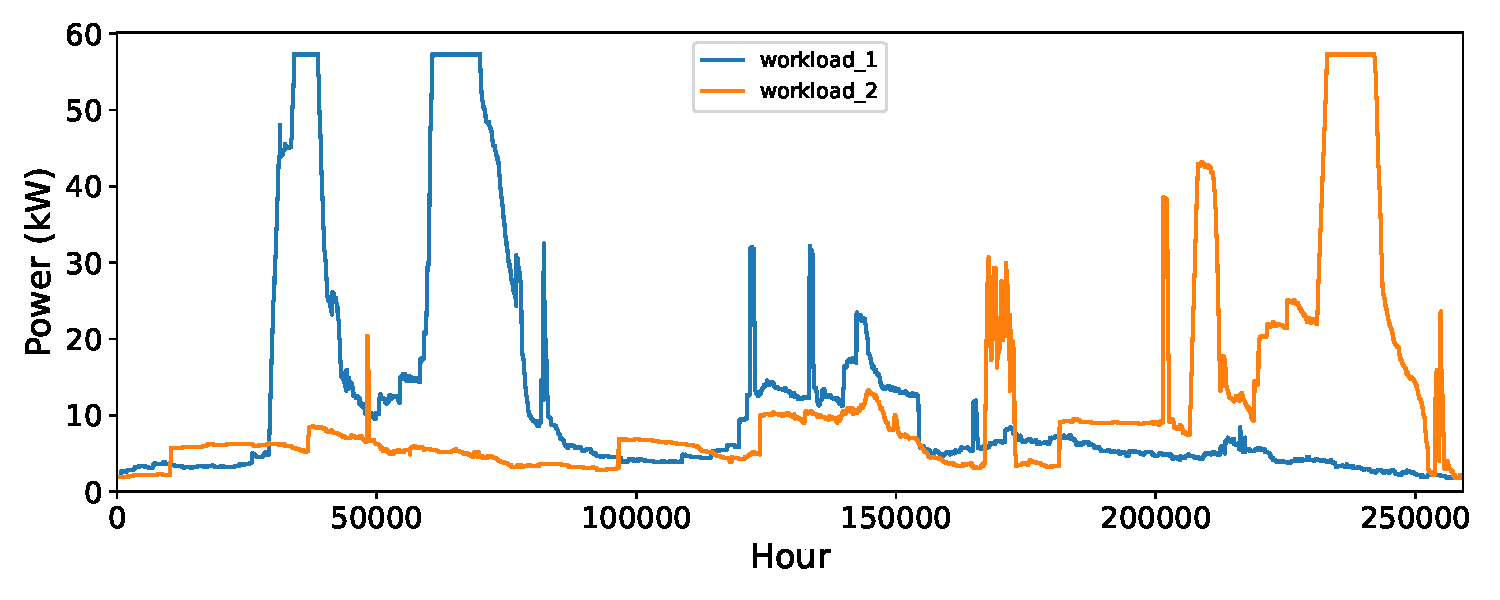
\includegraphics[scale=0.58]{Images/Compensations/critical_jobs_arriving.pdf}
    \caption{The power demanded for the critical scenarios.}
    \label{fig:critical_workload}
\end{figure}

We generated the weather data using MERRA and renewable ninja of 3 days for the \emph{critical scenarios}. Figure \ref{fig:critical_weather} shows the power production generated by the weather using the electrical components of our data center. 

\begin{figure}[!htb]
    \centering
    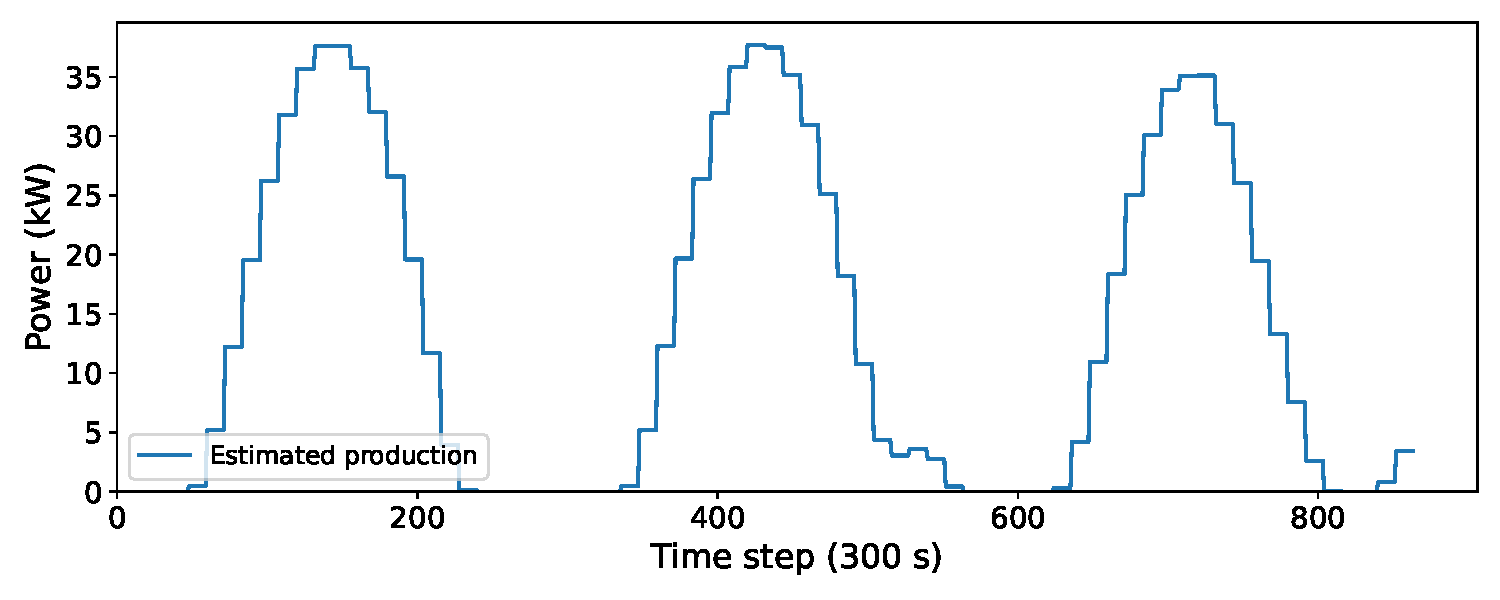
\includegraphics[scale=0.58]{Images/Compensations/critical_power_production.pdf}
    \caption{The power production for the critical scenarios.}
    \label{fig:critical_weather}
\end{figure}

We consider both workload and weather as predictions. Then, we use them to create an offline plan as presented in Section \ref{sec:offline_plan}. First, we solved the PDM model from Section \ref{sec:offline_modules} using the linearization proposed by \citeauthor{haddad2019mixed} \cite{haddad2019mixed}. Then, we took the production ($P_{prod}$) and solved the ITDM model. The ITDM model presented in Section \ref{sec:offline_modules} is too complex to solve a three-day time window with 400 servers. So, we simplified the problem, ignoring the transitions on$\rightarrow$off and off$\rightarrow$on. This new model returns the number of servers on and off at each time step and can be solved faster. After that, we have the offline plan. 

The next step is to introduce noise in the predictions to emulate the variations in reality. Every prediction provides a range of where the forecast is likely to be. So, we generated noises inside this range. In the critical scenarios, we considered that the range is $\pm 20\%$. Then, we created two new power productions: a worst-case and a best-case. In the worst-case scenario, all the productions are 20\% lower than predicted. On the other hand, in the best-case power production, all productions are 20\% higher. Figure \ref{fig:critical_weather_with_noise} illustrates the power production. Therefore, we simulated the worst and best cases of production (the reason for the name \emph{critical scenarios}).

\begin{figure}[!htb]
    \centering
    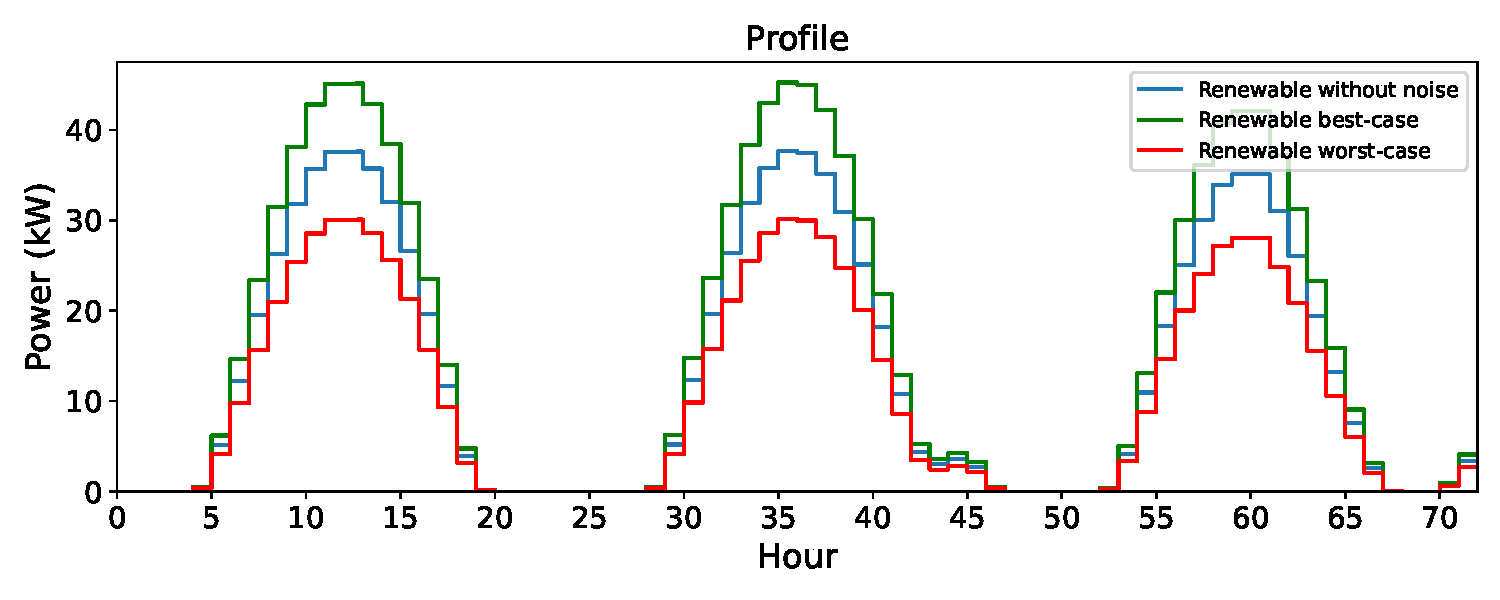
\includegraphics[scale=0.58]{Images/Compensations/critical_power_production_with_noise.pdf}
    \caption{The power production with noise for the critical scenarios.}
    \label{fig:critical_weather_with_noise}
\end{figure}

Regarding the workload, we introduced Gaussian noises in interarrival and job duration with a standard deviation of 20\% of the predicted value. The relation between these workload noises and the power demand is more complicated than the power production since the power demand depends on the scheduling algorithm and queue sort. Figure \ref{fig:critical_workload_with_noise} shows the impact of these noises on the power demand. Even if the impact on the workload power demand is not huge, these variances impact the offline IT plan since it will indicate the wrong moment to turn on/off the servers. The criticality of the workload comes from the moment where the jobs arrive (in the end or beginning).

\begin{figure}[!htb]
    \centering
    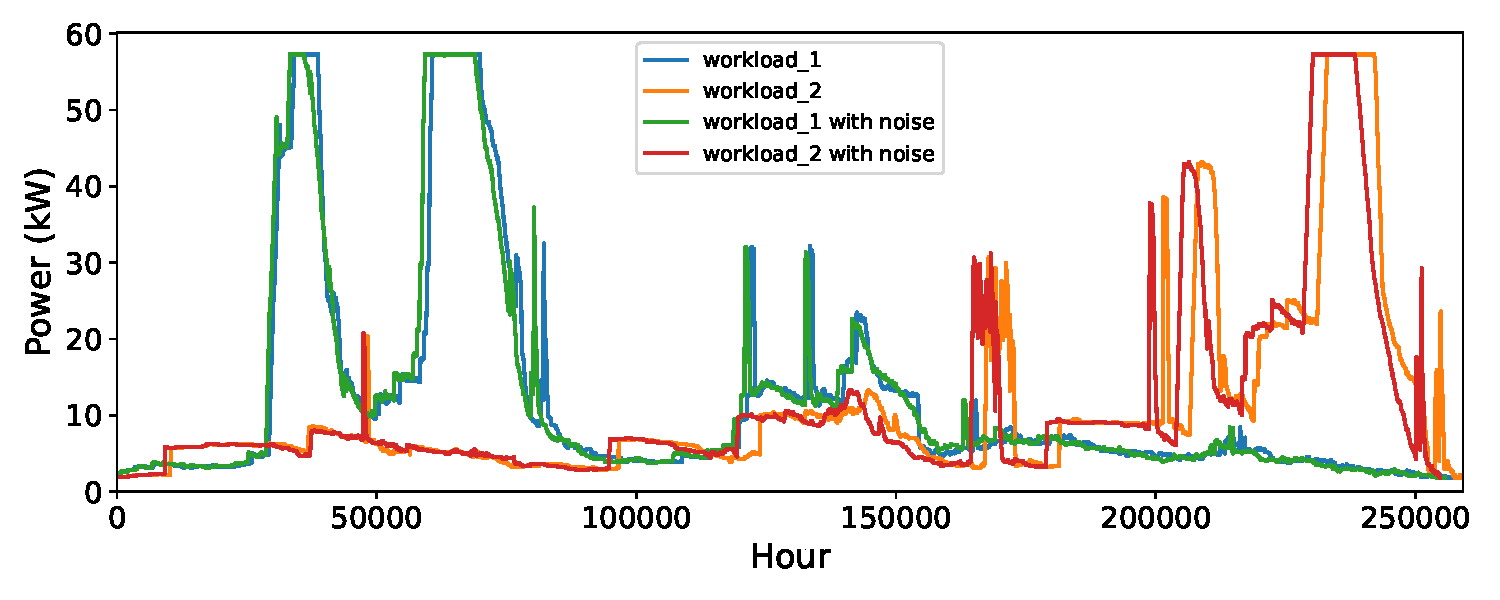
\includegraphics[scale=0.58]{Images/Compensations/critical_jobs_arriving_with_noise.pdf}
    \caption{The power demand with noise for the critical scenarios.}
    \label{fig:critical_workload_with_noise}
\end{figure}

Finally, we mixed the two productions (worst and best-case) with the two workloads (in the end and beginning), creating four scenarios:

\begin{enumerate}
    \item \emph{Critical 1}: Profile best-case and workload in the beginning;
    \item \emph{Critical 2}: Profile best-case and workload in the end;
    \item \emph{Critical 3}: Profile worst-case and workload in the beginning;
    \item \emph{Critical 4}: Profile worst-case and workload in the end;
\end{enumerate}

The first scenario is the best possible, with more energy and having all the jobs in the beginning. Therefore, the scheduler has the energy and time to decide when to place the jobs. However, the last scenario is the harder to make decisions, with lower energy and receiving the jobs at the very end.

\subsection{Average Scenarios}

In the \emph{Average Scenarios}, we chose 10 workload and weather traces. Figures \ref{fig:average_weather_with_noise} and \ref{fig:average_workload_with_noise} show the power production and demand, respectively. Then, we created 10 offline plans, one for each tuple of workload and profile. For example, workload 1 receives the production of profile 1, workload 2 receives profile 2, etc. The offline plans are created in the same way as the critical cases.

\begin{figure}[!htb]
    \centering
    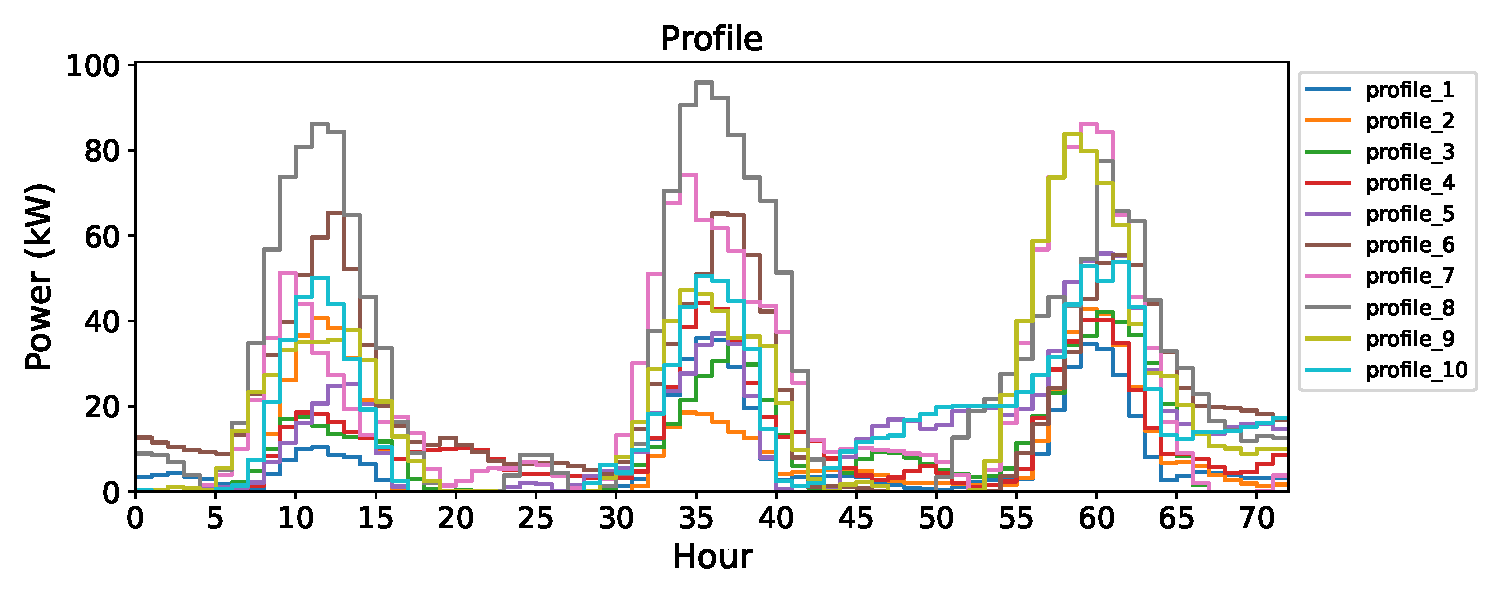
\includegraphics[scale=0.58]{Images/Compensations/diff_power_production.pdf}
    \caption{The power production for the average scenarios.}
    \label{fig:average_weather_with_noise}
\end{figure}

\begin{figure}[!htb]
    \centering
    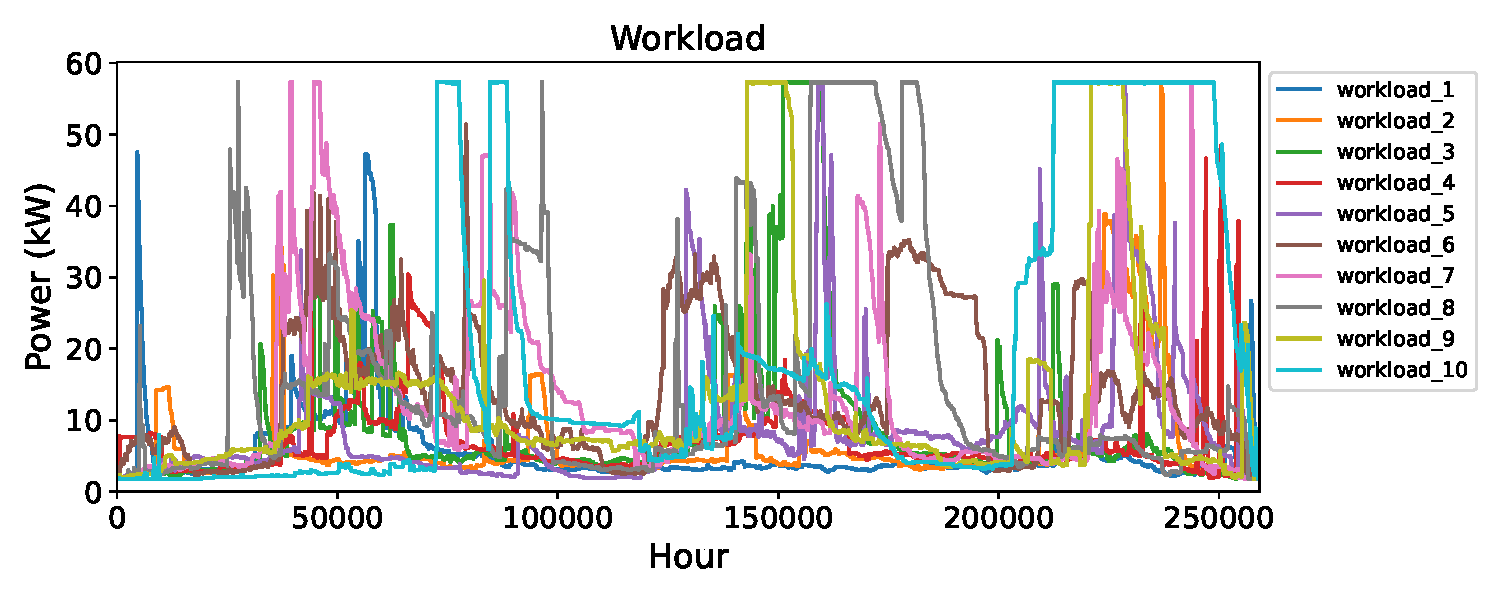
\includegraphics[scale=0.58]{Images/Compensations/diff_jobs_arriving.pdf}
    \caption{The power production for the average scenarios.}
    \label{fig:average_workload_with_noise}
\end{figure}

After creating the plans, we introduce noise in the values. Here, we applied Gaussian noises in power production, and jobs interarrival and size. We increase the standard deviation to 50\%, giving a larger range to generate values. Therefore, we have higher uncertainty. For each tuple (workload + profile), we generated 10 new workloads and profiles with noise, resulting in a total of 100 combinations. We called these scenarios as \emph{Average Scenarios} because they balance between positive and negative noises inside the same combination. In both parts (critical and average), besides the production and jobs noises, we have also the uncertainty from the walltime, presented in Section \ref{sec:workload_trace}.


\subsection{Baselines}
We created three baselines to compare the results from the four policies. The baselines are \emph{Follow plan}, \emph{Power reactive}, and \emph{Workload reactive}. \emph{Follow plan} is an algorithm that applies the offline plan without changing it. This algorithm emulates the execution of only the offline side. \emph{Power reactive} changes the server state according to the renewable power incoming. So, at each time step, it takes the power coming from renewable and calculates how many servers are possible to maintain running. It uses power from the batteries to maintain jobs running, if the renewable is not enough. \emph{Power reactive} uses the server configuration heuristic presented in Section \ref{sec:power_compensation}. \emph{Workload reactive} turns on the servers according to the job's arrival. It starts with all servers off. For each new job submitted, it turns on a server at maximum speed, if there is no server idle. After finishing a job, the server waits for $T_{wait}$ seconds (using the DPM technique from Equation \ref{equ:dpm_waiting_time}). If no job is placed on this server before $T_{wait}$, the scheduler sedates the server. In all cases (baselines and compensation policies), if the state of charge of the battery arrives at less than 20\% (defined $SoC_{min}$), the scheduler kills the jobs and sedates all servers. 

\section{Results Evaluation}

After describing the experimental environment, this section presents the results of the experiments. First, we discuss the critical cases. Then, we detail the results of the average cases.

\subsection{Critical cases}

\subsubsection{Scenario Critical 1}
Scenario Critical 1 (Profile best-case and workload in the beginning) is the case where the majority of jobs arrive at the beginning, and the production is higher than expected. However, this scenario is tricky. Since the battery starts with $SoC = 50\%$, if the scheduler starts too many jobs in the beginning, this can lead to a very low $SoC$ on the first day. This is exactly what happened with \emph{Workload reactive} in this scenario. Figure \ref{fig:DPM_soc} shows the evolution of the state of the charge in the \emph{Workload reactive} execution. At step 264 (79200 seconds after the simulation begins), \emph{Workload reactive} has less than 20\% of SoC. So, the scheduler kills the jobs. 

\begin{figure}[!htb]
    \centering
    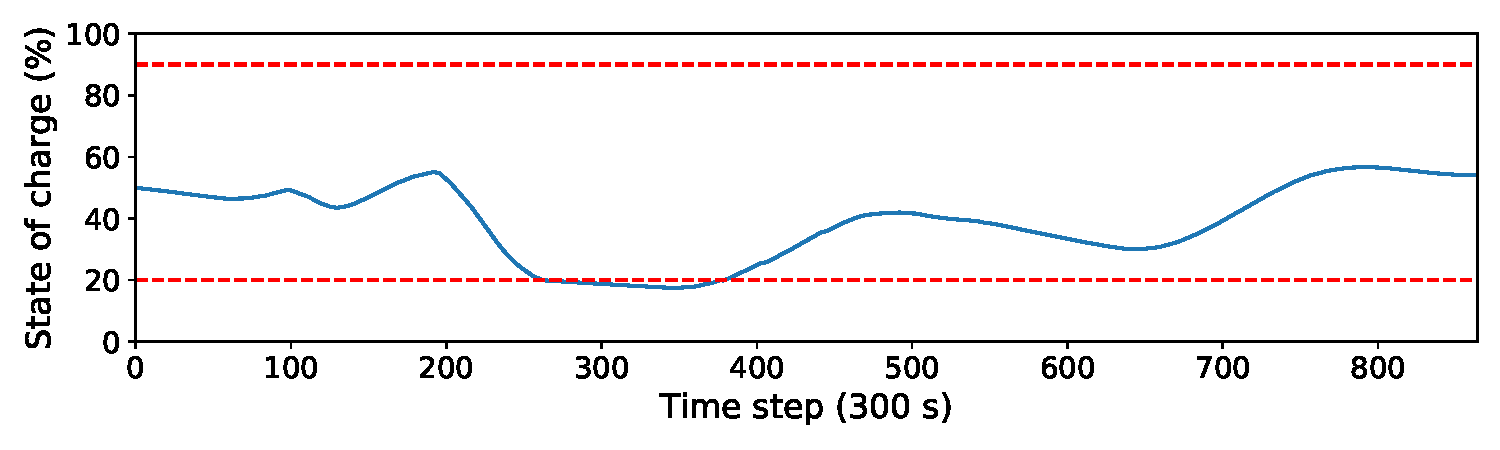
\includegraphics[scale=0.55]{Images/Compensations/critical_soc_s1.pdf}
    \caption{State of Charge for \emph{Workload reactive}.}
    \label{fig:DPM_soc}
\end{figure}

Figures \ref{fig:SoC_critical_1} and \ref{fig:jobs_critical_1} give the battery level at the end of the time window and jobs states, respectively. It is important to analyze both together. For example, \emph{Follow the plan} saves a lot of battery in this case, finishing with 20\% more energy than the target. This result seems very good, but analyzing the number of finished jobs, \emph{Follow the plan} has the lower finished jobs and higher killed jobs. This illustrates the importance of reacting to real events, using the saved energy to improve QoS. \emph{Power reactive} has the worst battery level, with an SoC of around 28\% (difference of -21.729269\%). This algorithm allocates all incoming power from renewable sources to servers, not recharging the battery. The battery recharges a little bit due to power fluctuations (e.g., the server is idle so the incoming renewable power recharges the battery instead of going to the server). So, it uses the battery to avoid killing jobs, but it does not compensate for this change. \emph{Power reactive} is the second-worst finished jobs metric, with some jobs reaching the walltime. Since it only uses the battery to avoid killing jobs, sometimes it let the servers at slower speeds, increasing the possibility of reaching walltime. It also kills some jobs because it also reaches the $SoC_{min}$.

\begin{figure}[!htb]
    \centering
    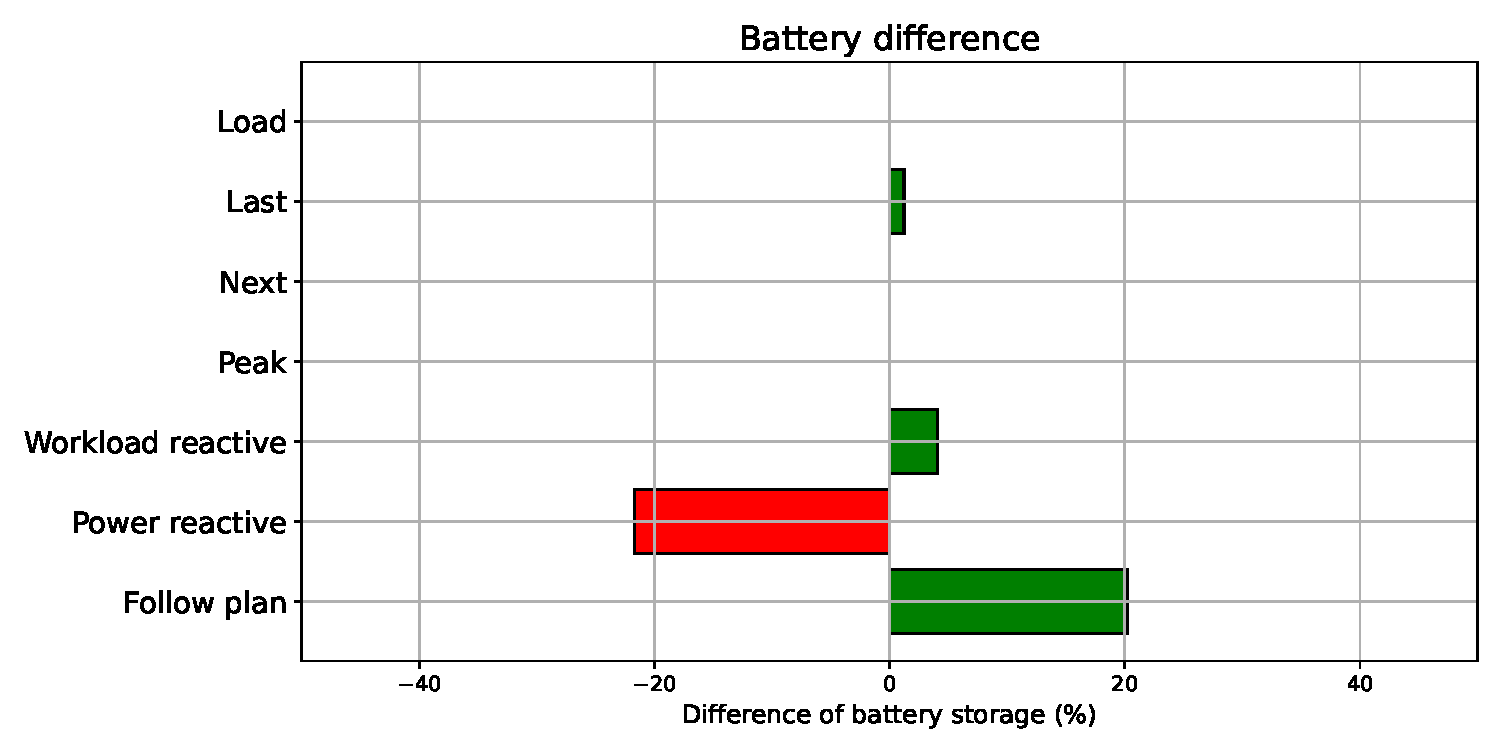
\includegraphics[scale=0.55]{Images/Compensations/battery_critical_1.pdf}
    \caption{Difference between the battery target level (50\%) and the real battery level at the end of the time window for scenario critical 1.}
    \label{fig:SoC_critical_1}
\end{figure}

\begin{figure}[!htb]
    \centering
    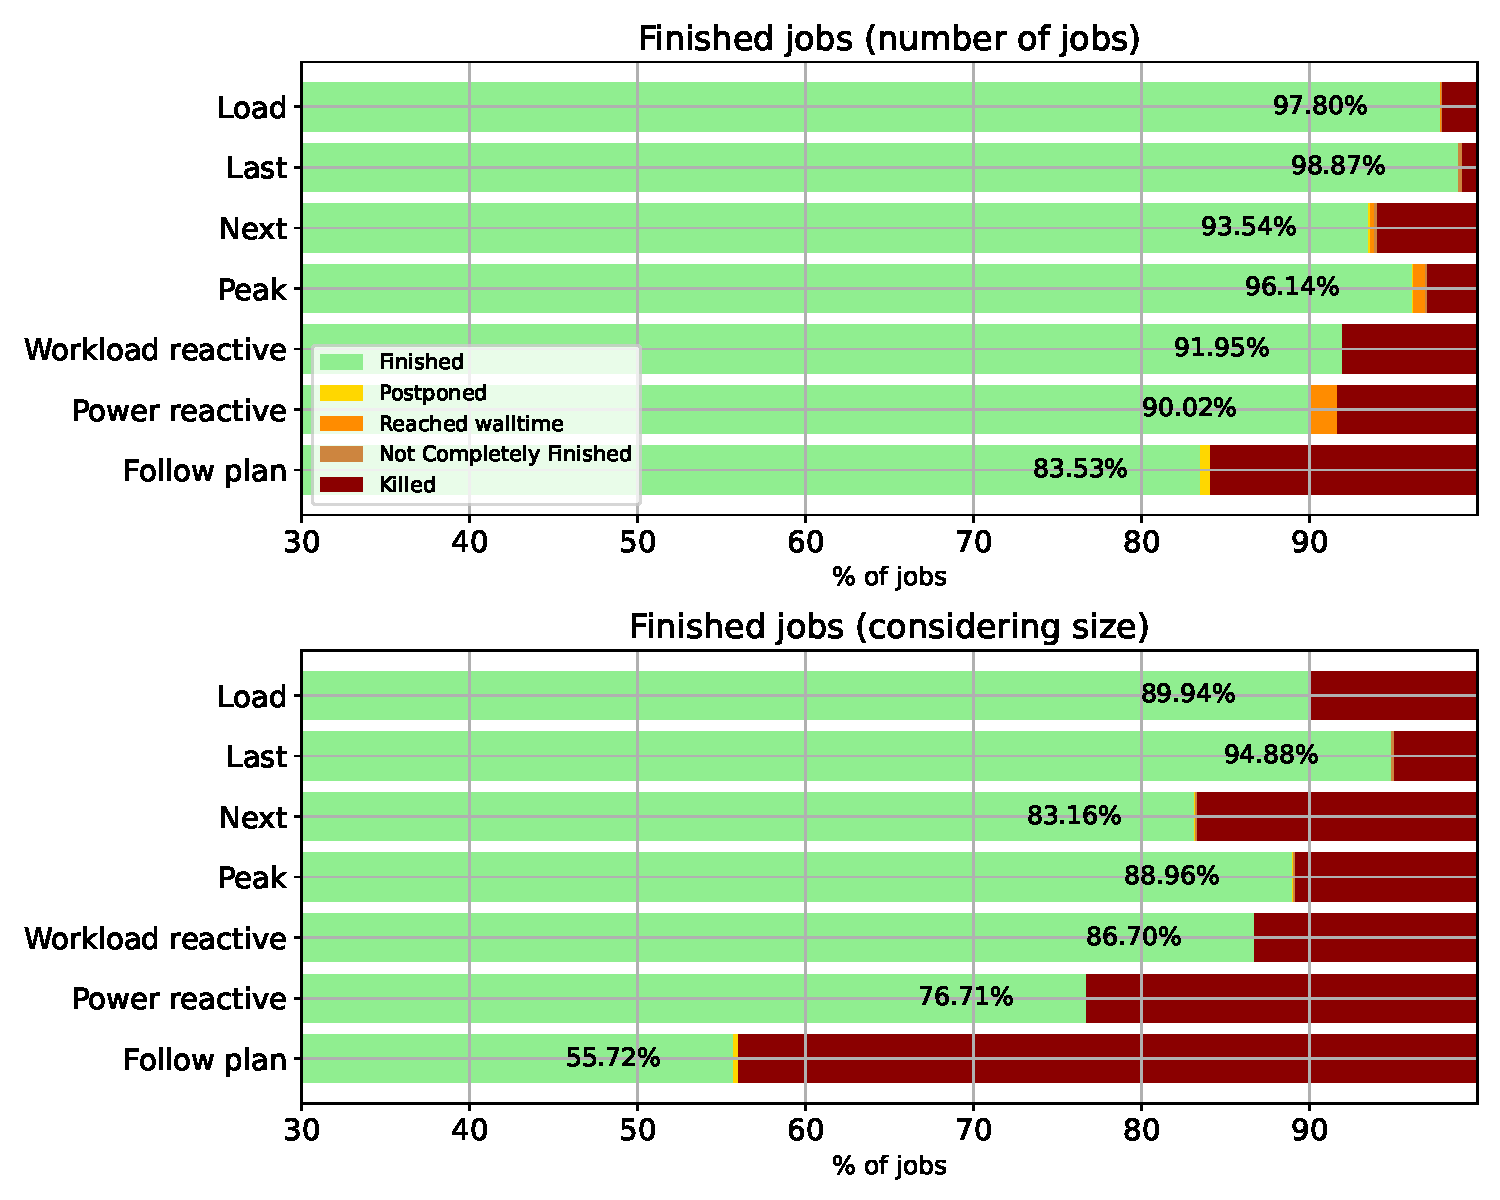
\includegraphics[scale=0.55]{Images/Compensations/jobs_critical_1.pdf}
    \caption{Jobs states at scenario critical 1.}
    \label{fig:jobs_critical_1}
\end{figure}

As mentioned at the beginning of this section, \emph{Workload reactive} can not manage well the state of charge, killing some jobs. Even so, it finishes with a good battery level. The DPM technique helps to save some energy, letting the incoming renewable to recharge the battery. Since it always put the servers at maximum speed, no job reached the walltime. It has the third-worst finished and killed jobs. All the policies are very close to the target level. Just \emph{Last} policy saved a little bit more than the target, because it puts all the compensations in the end, and it can not use everything. Considering the metrics about the job, all policies finished more jobs and killed less than the three baselines. The best one is \emph{Last} with 98.87\% of the finished jobs, and the lowest killed jobs. \emph{Load} places the compensations in the steps where it is expected to have higher demand. In this case, it pays off with the second-best results. We will see in future cases that this behavior is dangerous. 

\emph{Next} has the worst job result among the policies. This result can be explained by comparing \emph{Next} and \emph{Last}. For example, let's say we saved energy in step 0. So, \emph{Last} increase the usage in the last possible step. If at any moment between step 0 and the last step, it is necessary to use more energy, \emph{Last} can take the previous migration and use it now. On the other hand, \emph{Next} expended this energy as soon as possible. Therefore, \emph{Next} can arrive in some moments without energy to avoid killing jobs. Finally, \emph{Peak} has the third-best result, but with some jobs reaching the walltime. Since it shaves the power usage (negative/positive) peaks, it can reduce speed in critical moments (e.g., with a lot of jobs running). 

The second analysis is regarding wasted energy. Figure \ref{fig:energy_critical_1} shows the results. \emph{Workload reactive} turns on resources on demand and does not let idle servers available too much. Therefore, it has the best wasted energy metric compared with the other algorithms. The worst case is \emph{Power reactive} which turns on servers according to the power available and not the demand. \emph{Follow the plan} and the four policies are guided by the offline plan. Therefore, the noise introduced in the real workload can lead to some mismatch between demand and production. Since \emph{Follow the plan} kills more jobs than the policies, this metric is higher for this algorithm. The energy expended in killed jobs is considered wasted energy since the result of the killed job is useless. \emph{Last} has the second-best wasted energy since it runs more jobs than the other algorithms.

\begin{figure}[!htb]
    \centering
    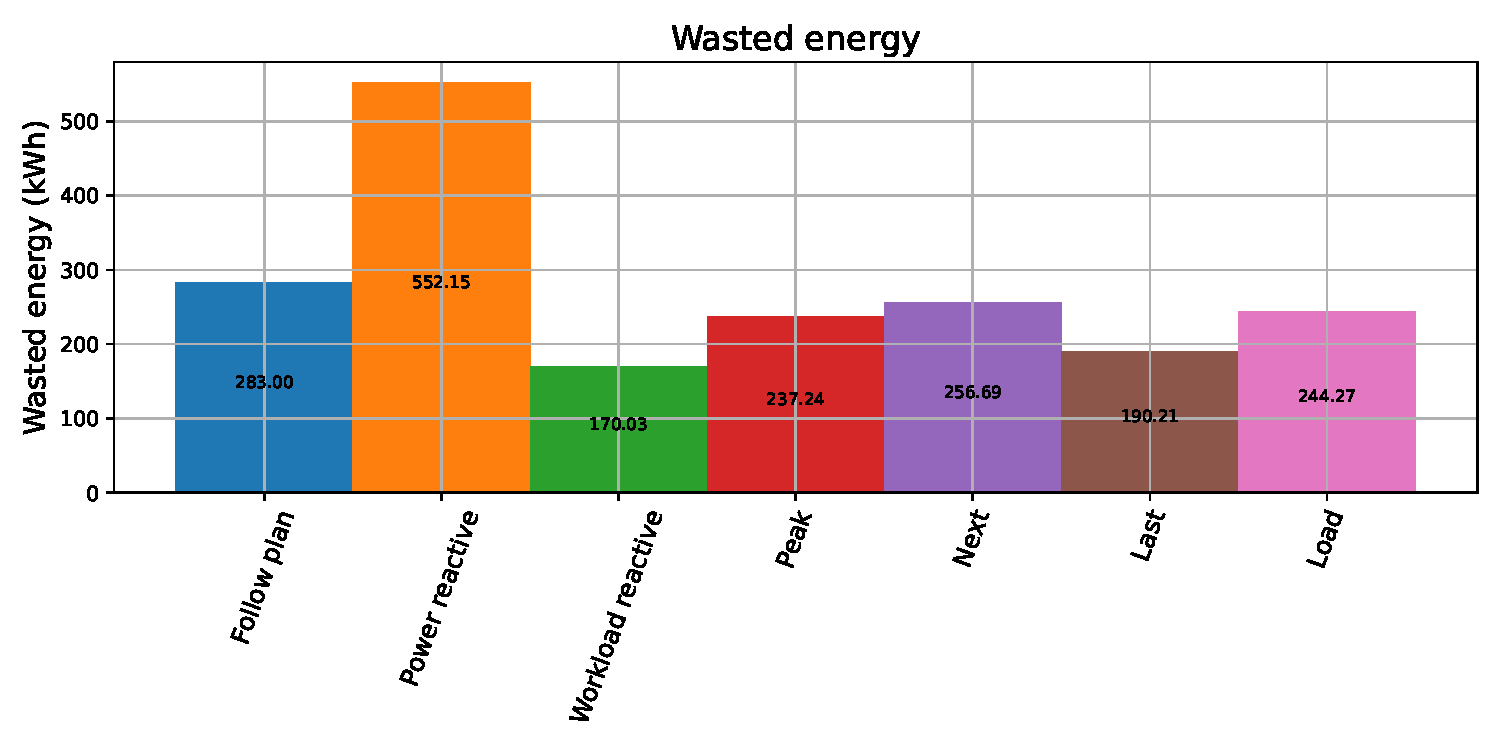
\includegraphics[scale=0.55]{Images/Compensations/energy_critical_1.pdf}
    \caption{Wasted energy at scenario critical 1.}
    \label{fig:energy_critical_1}
\end{figure}

Finally, Figure \ref{fig:slowdown_critical_1} demonstrates the slowdown of the finished jobs. As mentioned before, this metric is complicated to compare in an experiment with different numbers of finished jobs. We can see that \emph{Workload reactive} has some jobs with very high slowdown. It happens because stays a long period with the SoC below $SoC_{min}$ (as illustrated in Figure \ref{fig:DPM_soc}). So, it has a long period without servers running. \emph{Load} has a good mean and median. In this case, \emph{Load} can place the compensations close to the jobs' arrival. 

\begin{figure}[!htb]
    \centering
    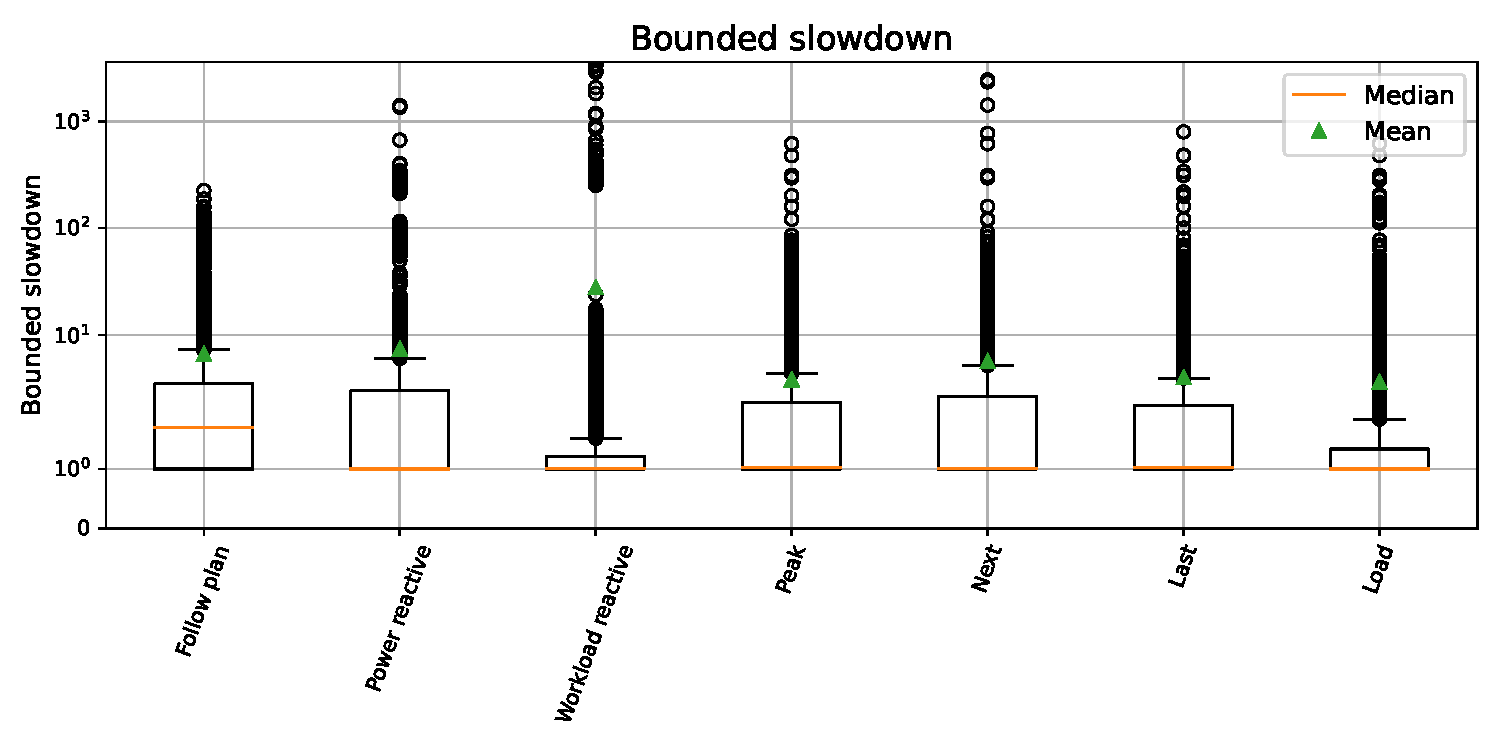
\includegraphics[scale=0.55]{Images/Compensations/slowdown_critical_1.pdf}
    \caption{Bounded slowdown at scenario critical 1.}
    \label{fig:slowdown_critical_1}
\end{figure}

\clearpage

\subsubsection{Scenario Critical 2}

Scenario Critical 2 has more energy than predicted (Profile best-case) and the jobs arriving in the end. In this scenario, the policies do not have much time to compensate, since the load comes on the last day. 

\begin{figure}[!htb]
    \centering
    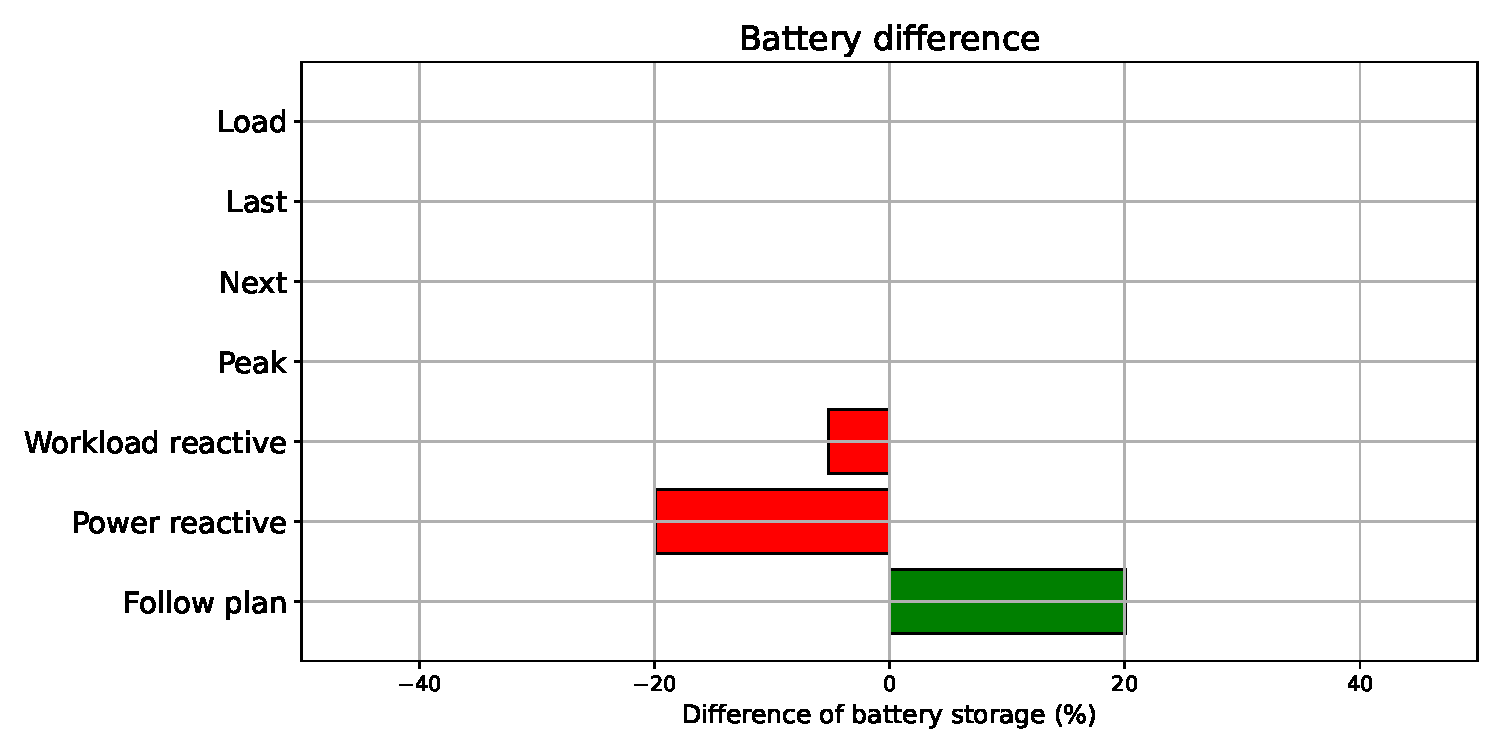
\includegraphics[scale=0.55]{Images/Compensations/battery_critical_2.pdf}
    \caption{Difference between the battery target level (50\%) and the real battery level at the end of the time window for scenario critical 2.}
    \label{fig:SoC_critical_2}
\end{figure}

\begin{figure}[!htb]
    \centering
    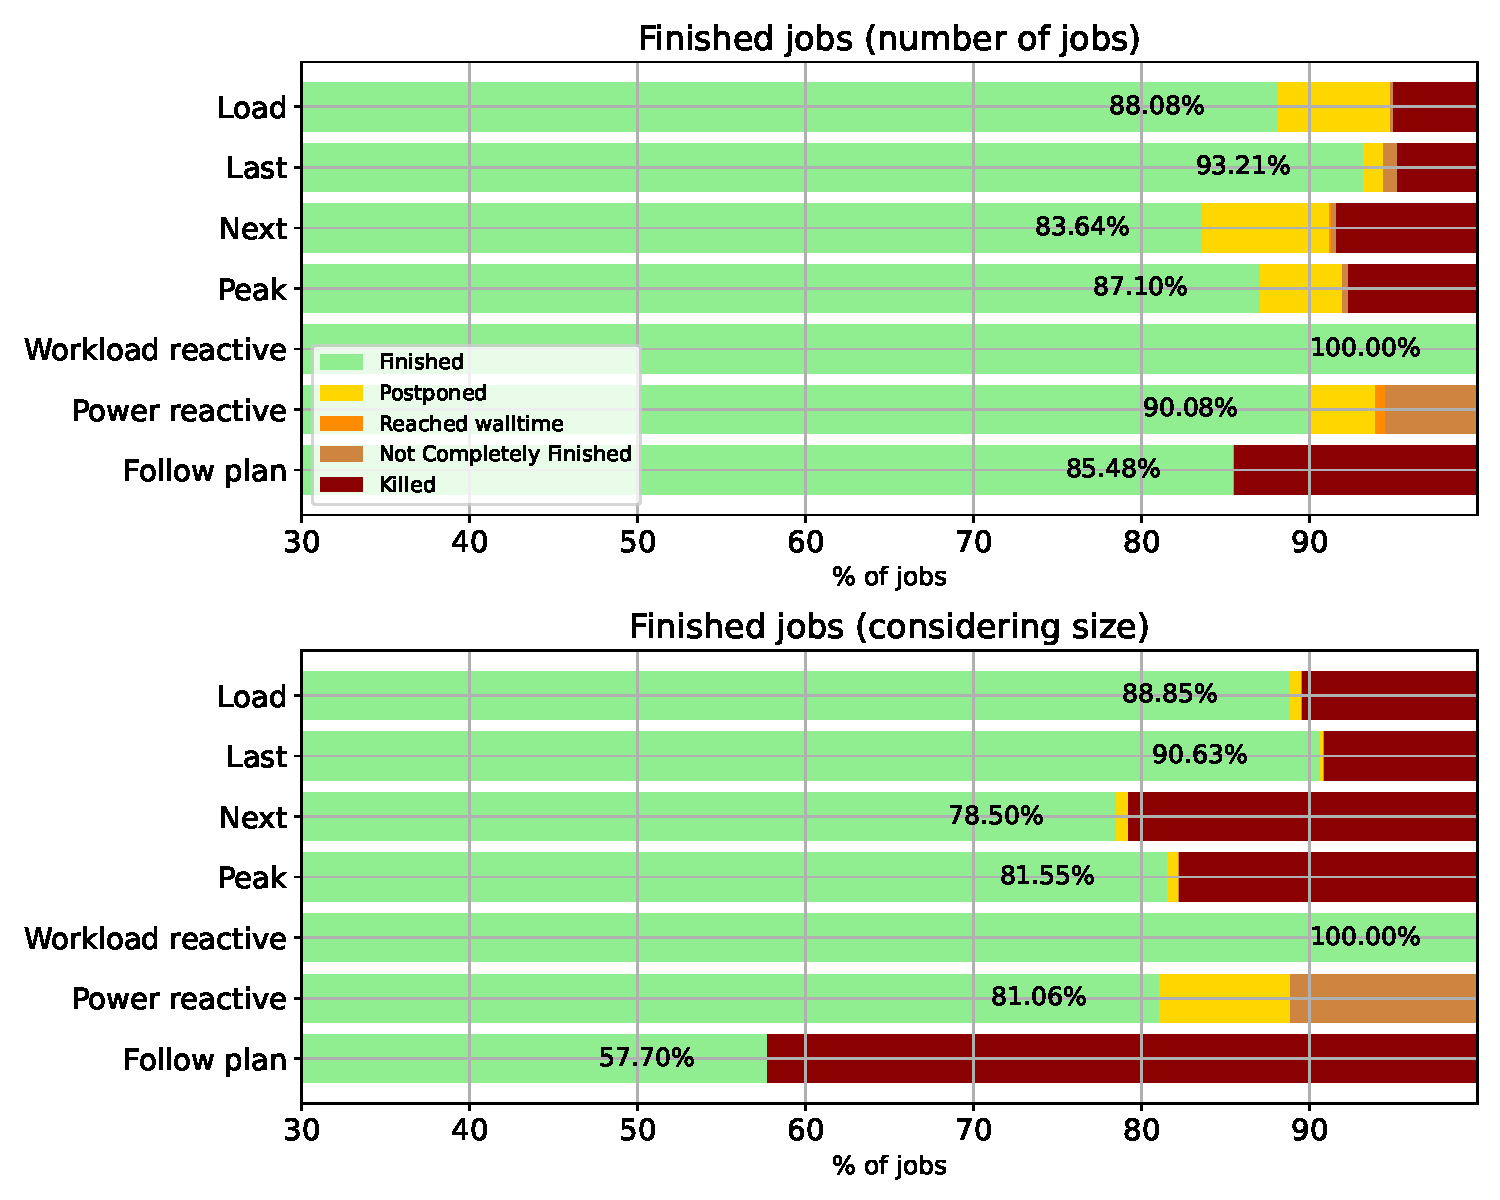
\includegraphics[scale=0.55]{Images/Compensations/jobs_critical_2.pdf}
    \caption{Jobs state at scenario Critical 2.}
    \label{fig:jobs_critical_2}
\end{figure}

\begin{figure}[!htb]
    \centering
    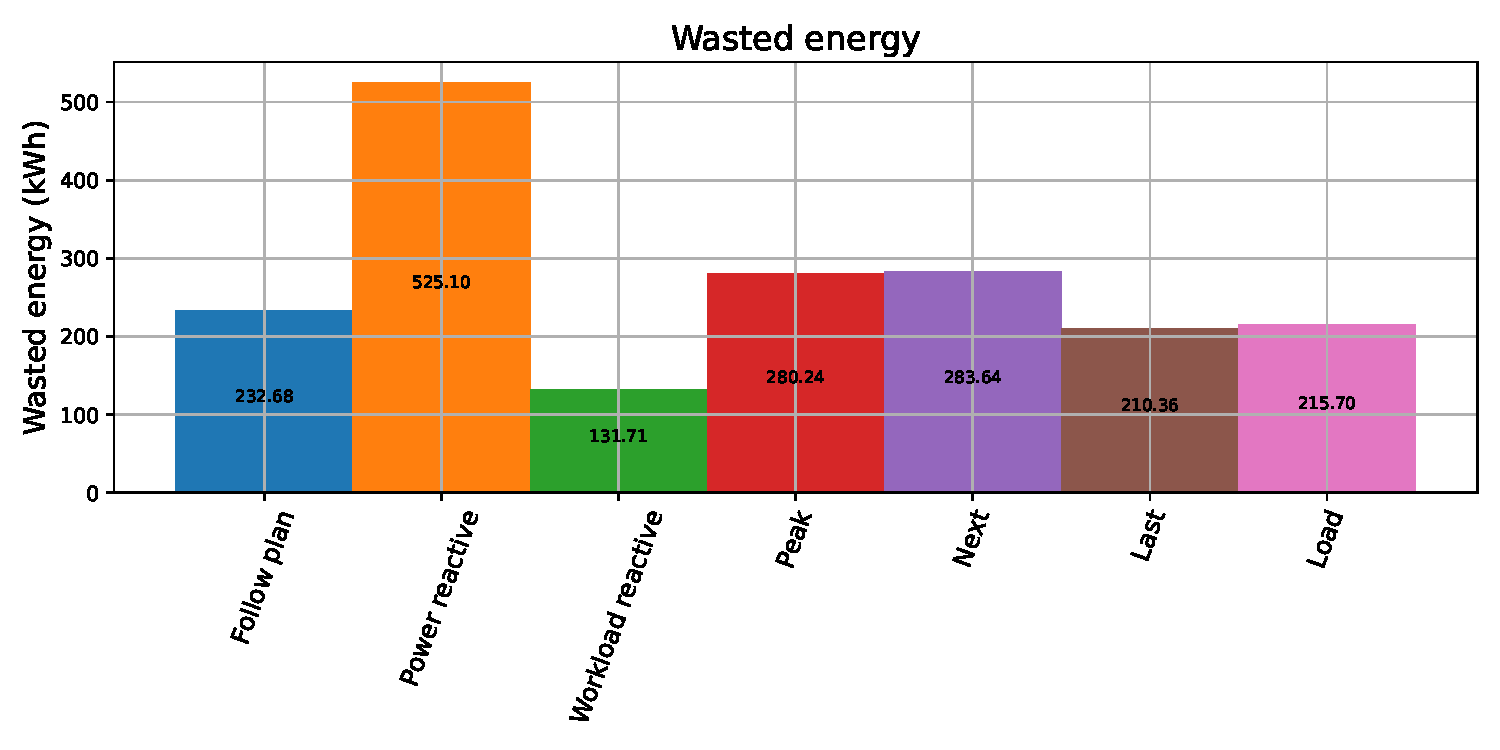
\includegraphics[scale=0.55]{Images/Compensations/energy_critical_2.pdf}
    \caption{Wasted energy at scenario Critical 2.}
    \label{fig:energy_critical_2}
\end{figure}

\begin{figure}[!htb]
    \centering
    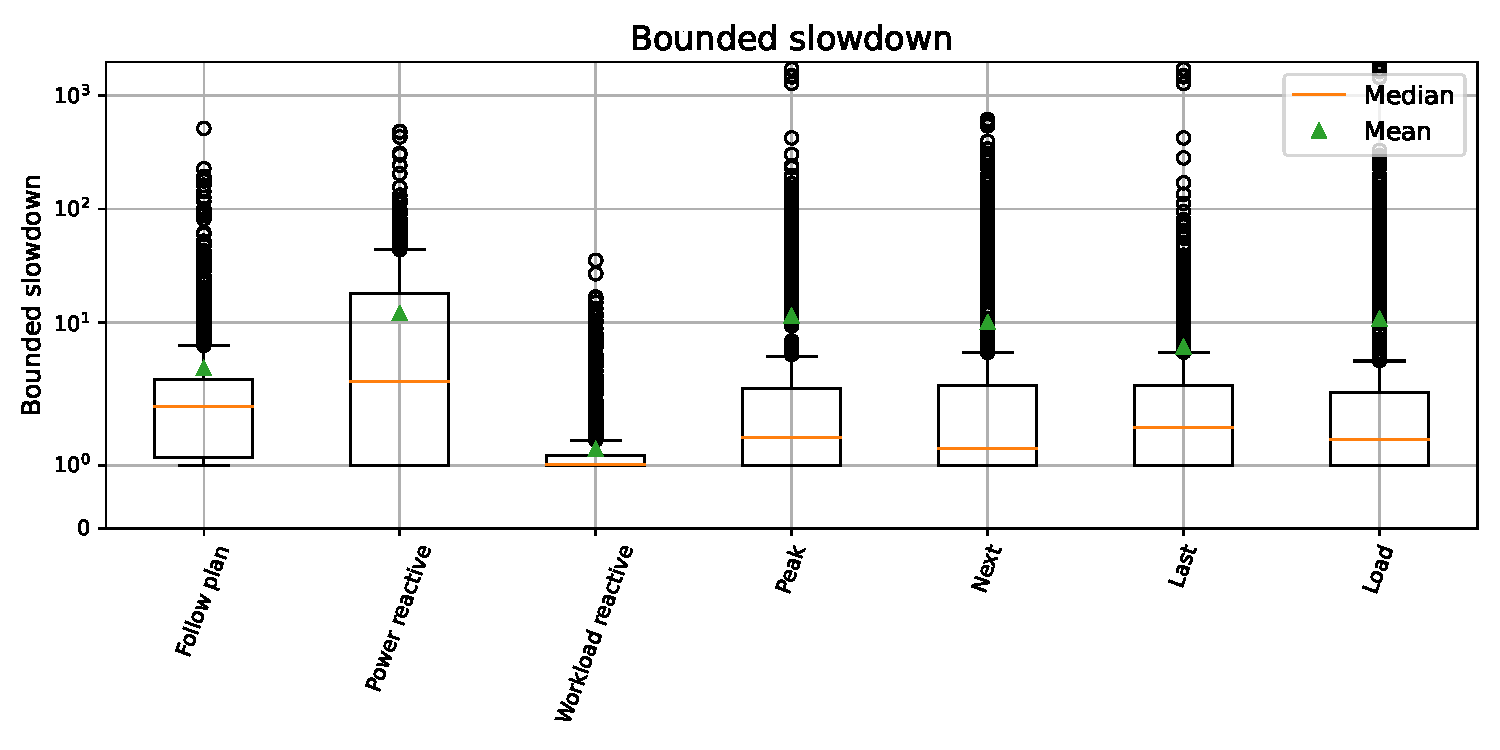
\includegraphics[scale=0.55]{Images/Compensations/slowdown_critical_2.pdf}
    \caption{Bounded slowdown at scenario Critical 2.}
    \label{fig:slowdown_critical_2}
\end{figure}

\clearpage

\subsubsection{Scenario Critical 3}

\begin{figure}[!htb]
    \centering
    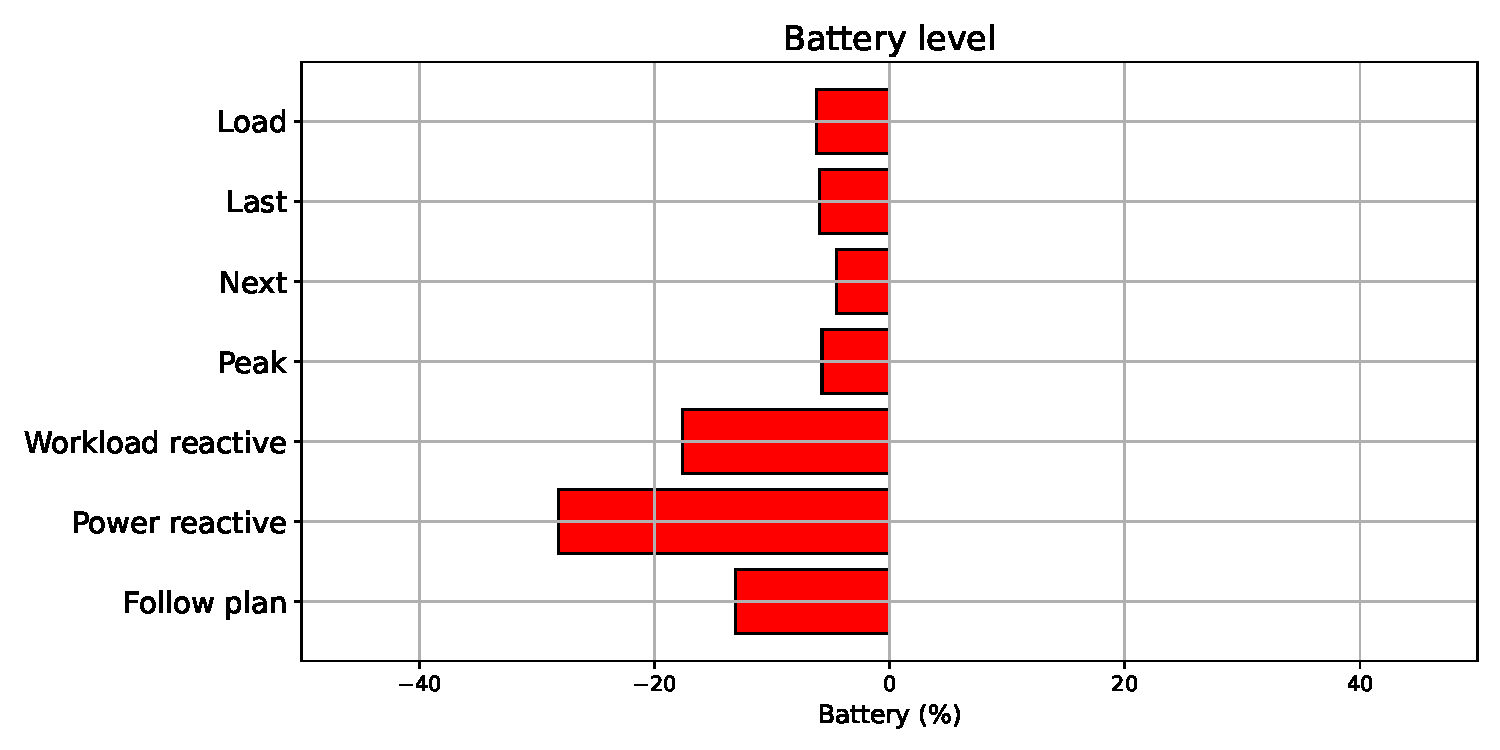
\includegraphics[scale=0.55]{Images/Compensations/battery_critical_3.pdf}
    \caption{Difference between the battery target level (50\%) and the real battery level at the end of the time window for scenario critical 3.}
    \label{fig:SoC_critical_3}
\end{figure}

\begin{figure}[!htb]
    \centering
    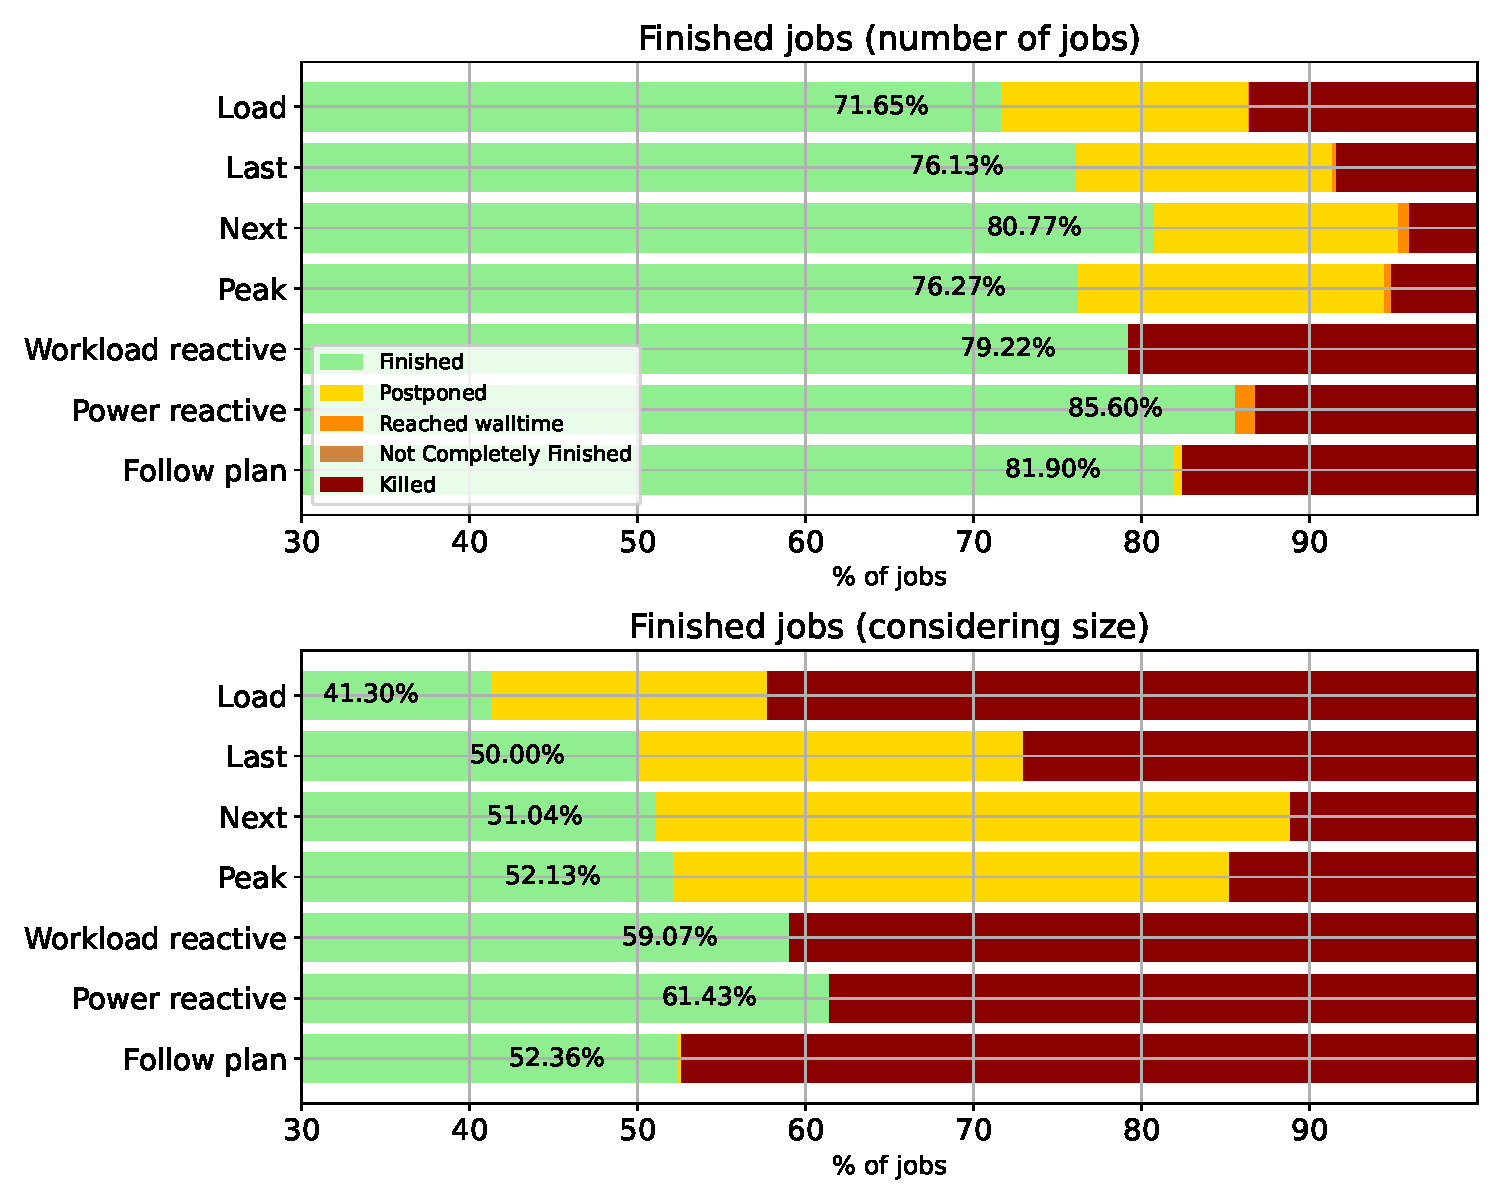
\includegraphics[scale=0.55]{Images/Compensations/jobs_critical_3.pdf}
    \caption{Jobs state at scenario critical 3.}
    \label{fig:jobs_critical_3}
\end{figure}

\begin{figure}[!htb]
    \centering
    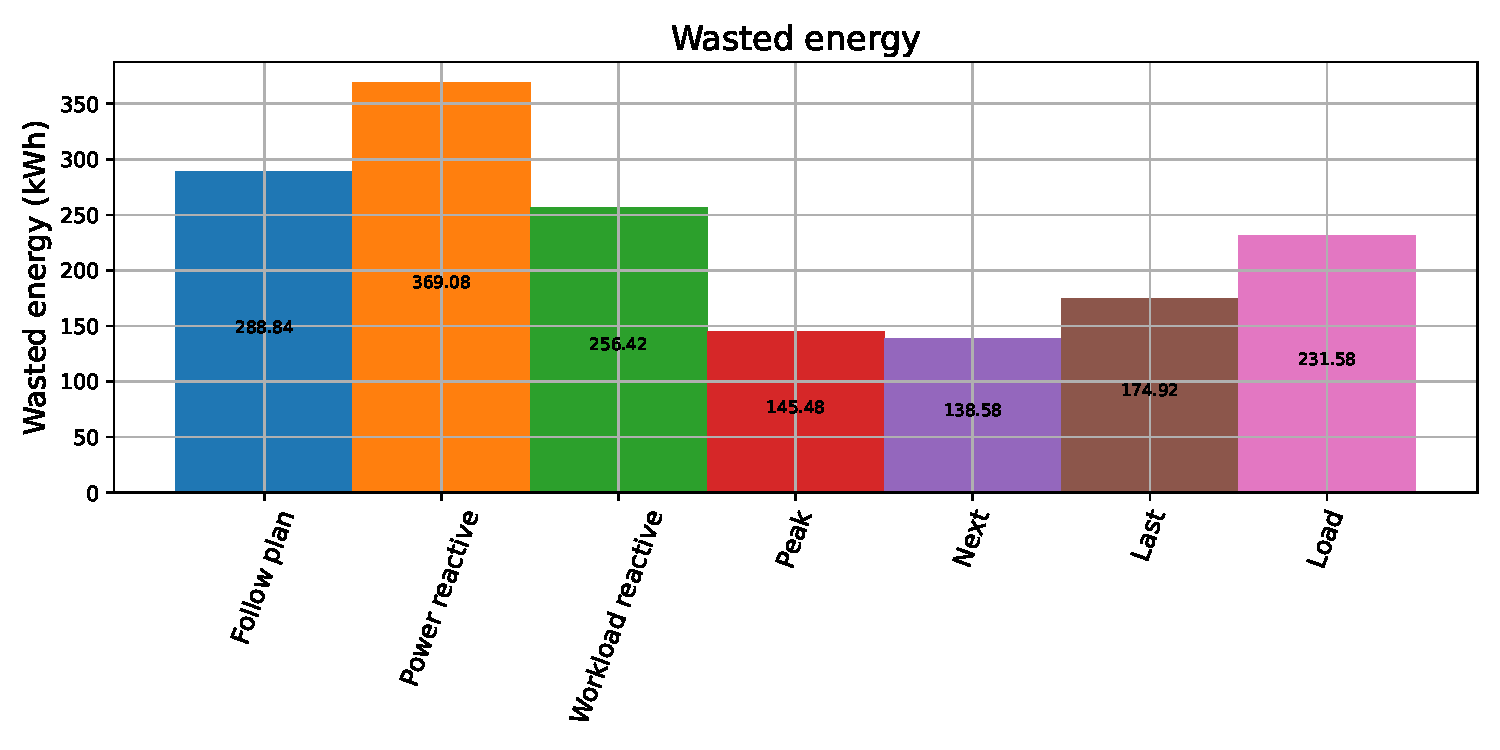
\includegraphics[scale=0.55]{Images/Compensations/energy_critical_3.pdf}
    \caption{Wasted energy at scenario critical 3.}
    \label{fig:energy_critical_3}
\end{figure}

\begin{figure}[!htb]
    \centering
    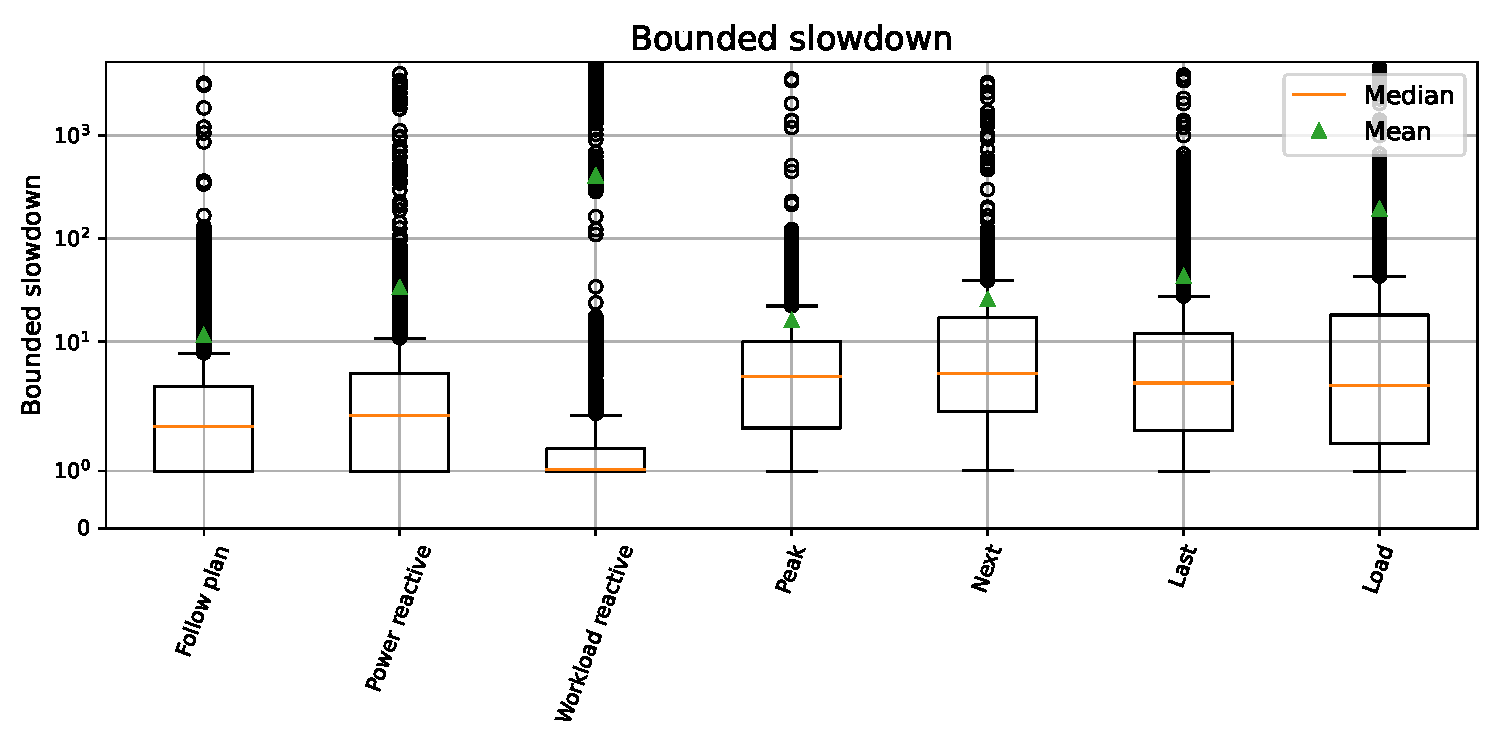
\includegraphics[scale=0.55]{Images/Compensations/slowdown_critical_3.pdf}
    \caption{Bounded slowdown at scenario critical 3.}
    \label{fig:slowdown_critical_3}
\end{figure}

\clearpage

\subsubsection{Scenario Critical 4}

\begin{figure}[!htb]
    \centering
    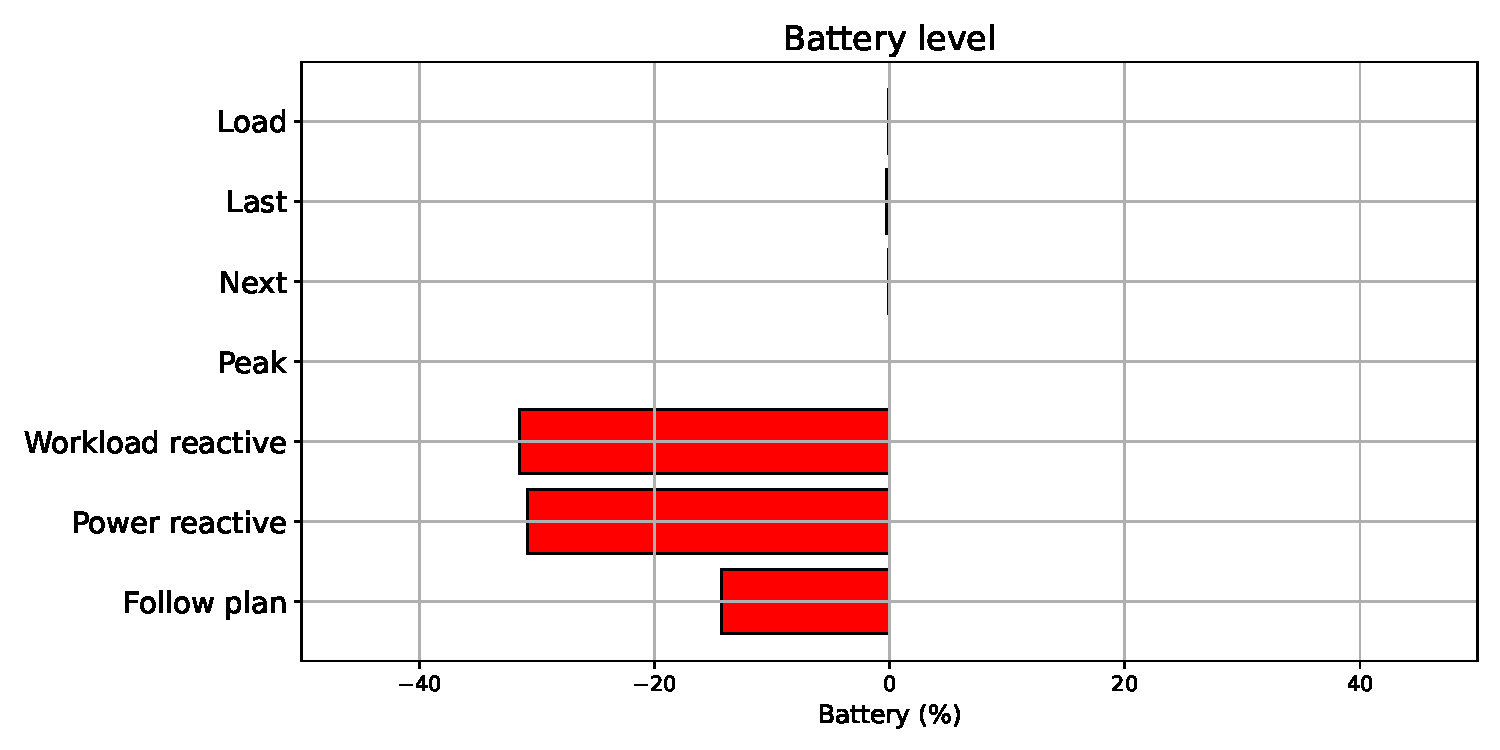
\includegraphics[scale=0.55]{Images/Compensations/battery_critical_4.pdf}
    \caption{Difference between the battery target level (50\%) and the real battery level at the end of the time window for scenario critical 4.}
    \label{fig:SoC_critical_4}
\end{figure}

\begin{figure}[!htb]
    \centering
    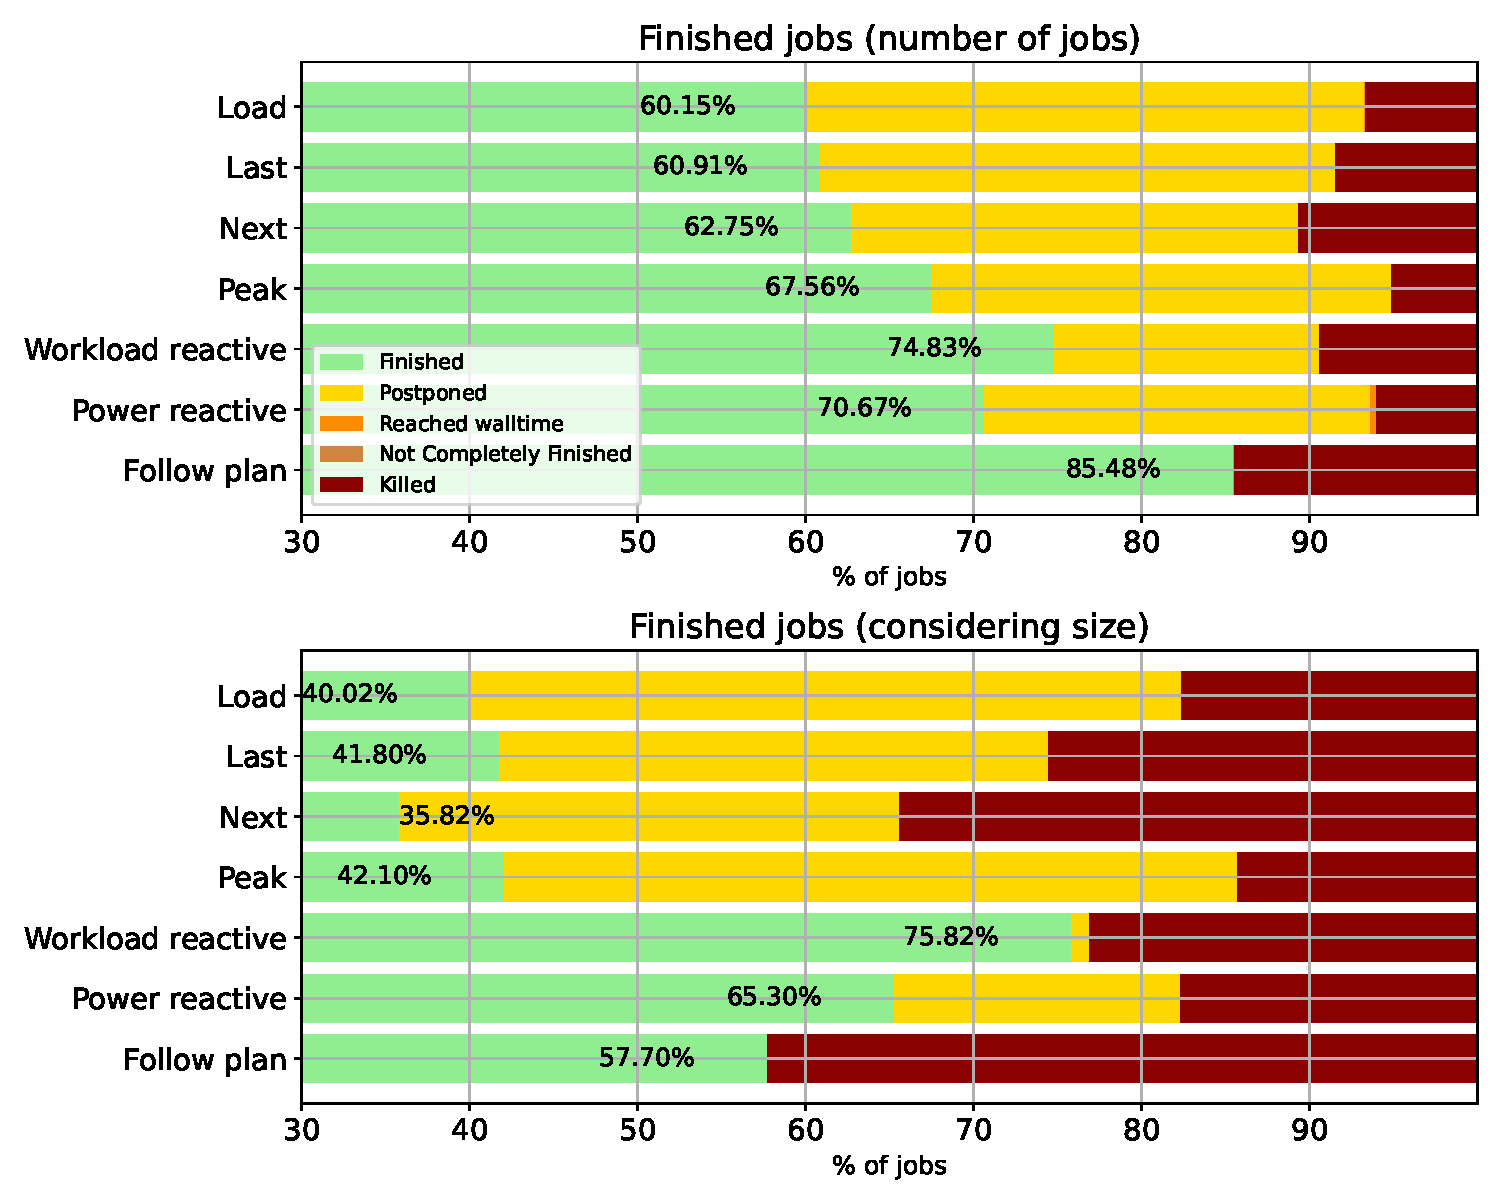
\includegraphics[scale=0.55]{Images/Compensations/jobs_critical_4.pdf}
    \caption{Jobs state at scenario critical 4.}
    \label{fig:jobs_critical_4}
\end{figure}

\begin{figure}[!htb]
    \centering
    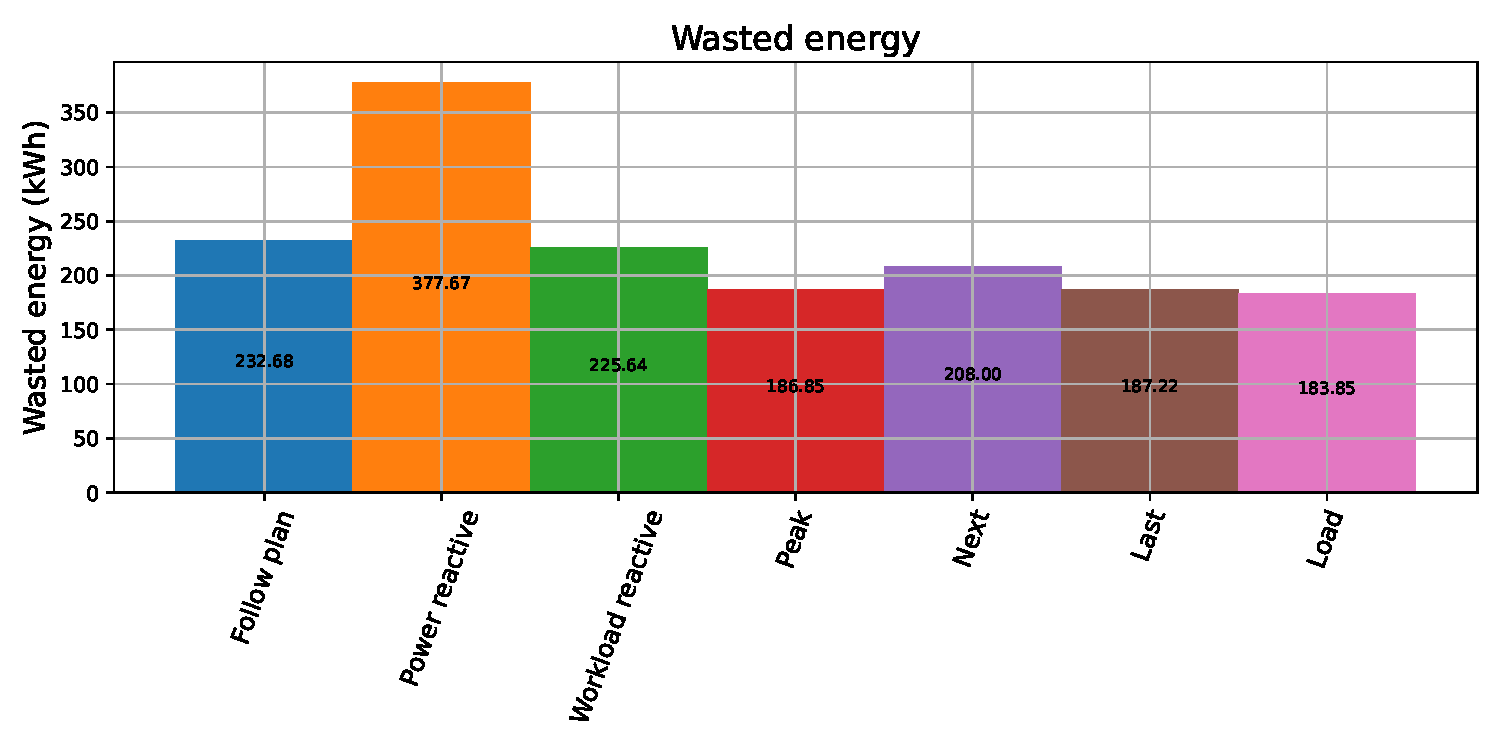
\includegraphics[scale=0.55]{Images/Compensations/energy_critical_4.pdf}
    \caption{Wasted energy at scenario critical 4.}
    \label{fig:energy_critical_4}
\end{figure}

\begin{figure}[!htb]
    \centering
    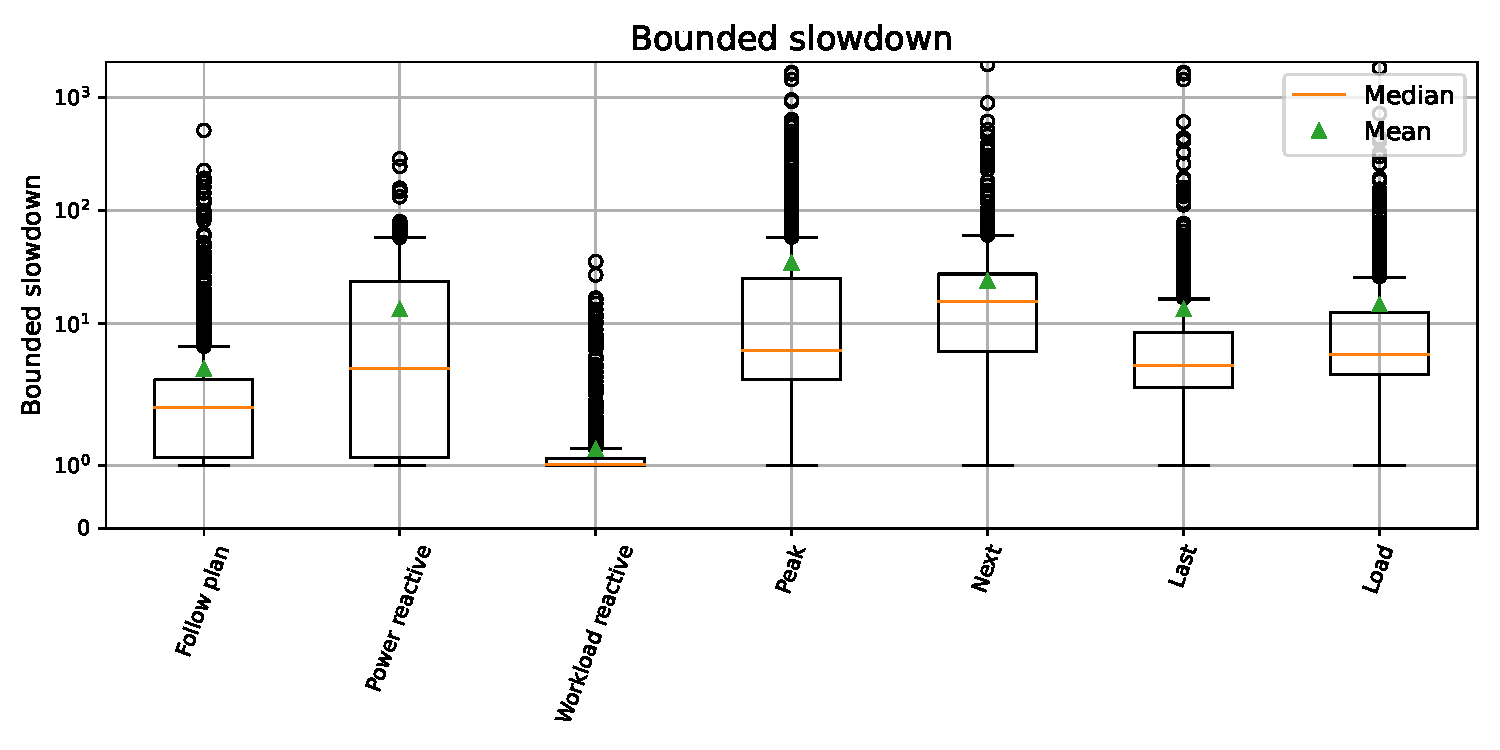
\includegraphics[scale=0.55]{Images/Compensations/slowdown_critical_4.pdf}
    \caption{Bounded slowdown at scenario critical 4.}
    \label{fig:slowdown_critical_4}
\end{figure}

\clearpage

\subsection{Average cases}

\begin{figure}[!htb]
    \centering
    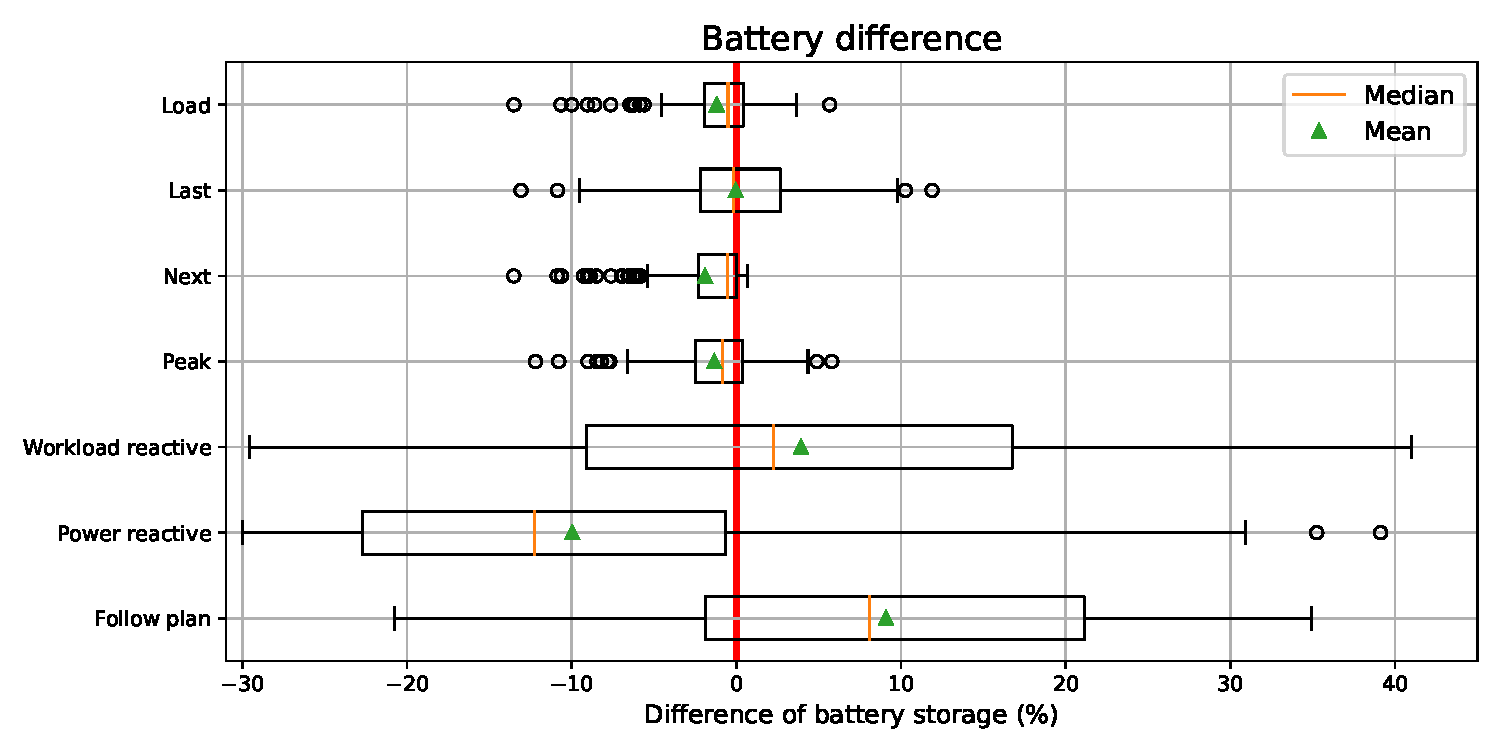
\includegraphics[scale=0.55]{Images/Compensations/battery_diff.pdf}
    \caption{Difference between the battery target level (50\%) and the real battery level at the end of the time window at 100 average cases. The line shows the standard deviation.}
    \label{fig:SoC_diff}
\end{figure}

\begin{figure}[!htb]
    \centering
    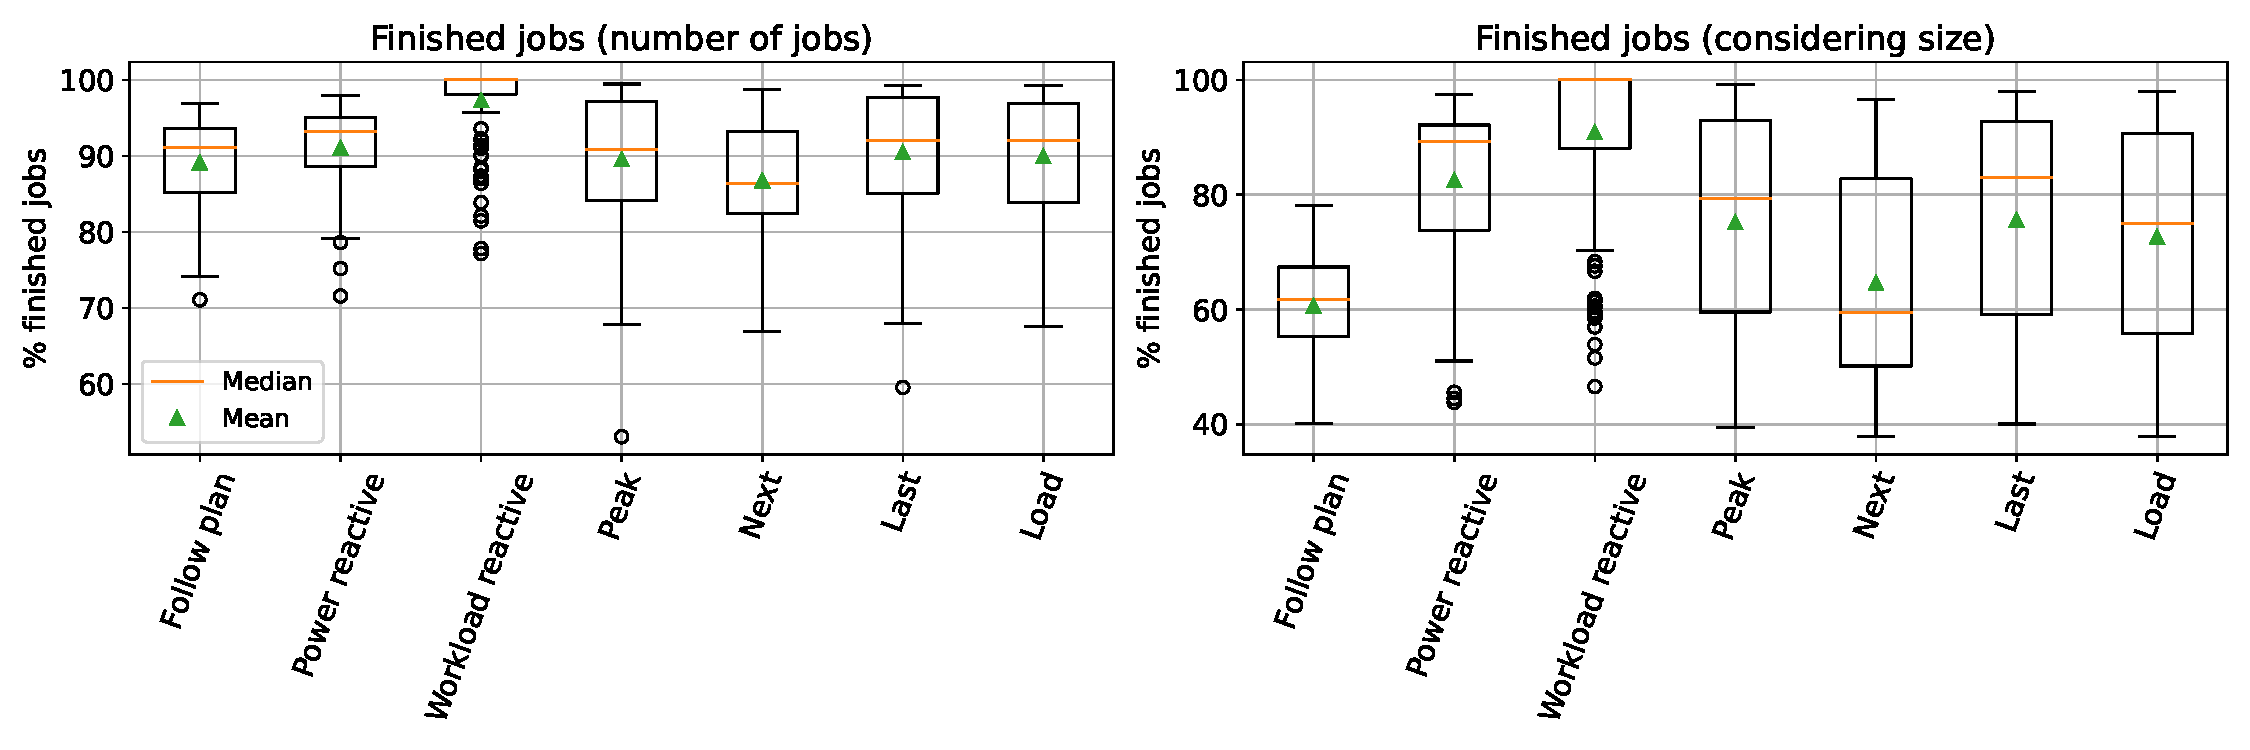
\includegraphics[scale=0.55]{Images/Compensations/finished_diff.pdf}
    \caption{Finished jobs at 100 average cases.}
    \label{fig:finished_diff}
\end{figure}

\begin{figure}[!htb]
    \centering
    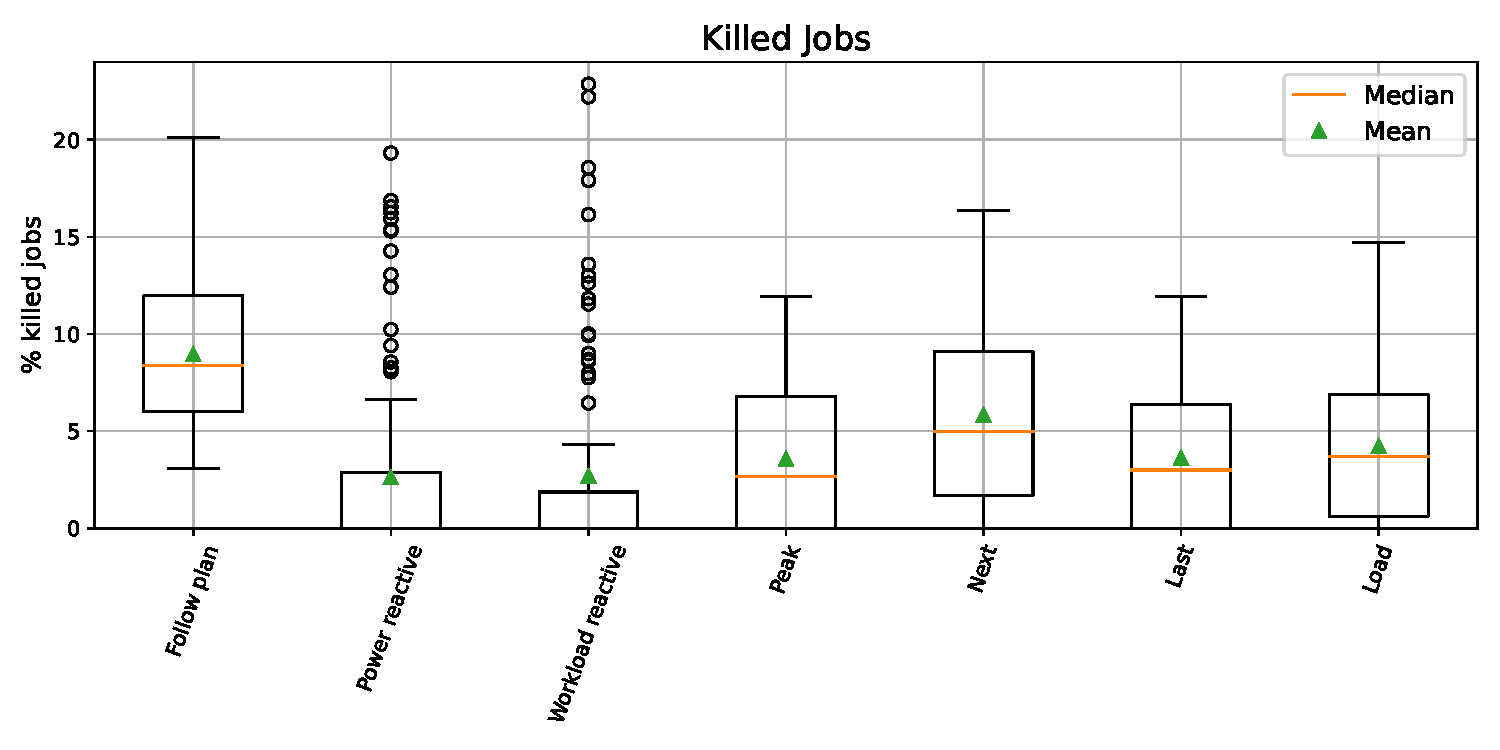
\includegraphics[scale=0.55]{Images/Compensations/killed_diff.pdf}
    \caption{Killed jobs at 100 average cases.}
    \label{fig:killed_diff}
\end{figure}

\begin{figure}[!htb]
    \centering
    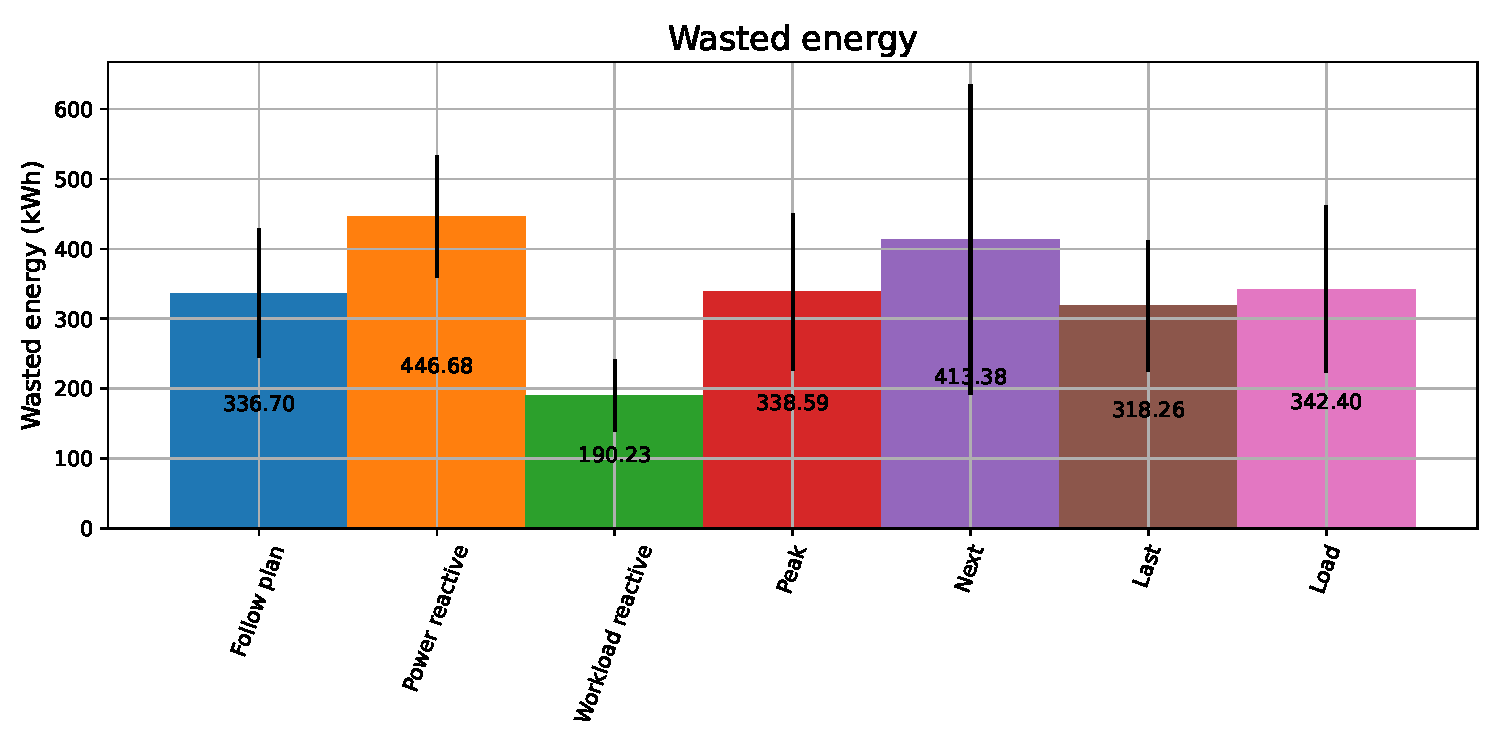
\includegraphics[scale=0.55]{Images/Compensations/energy_diff.pdf}
    \caption{Wasted energy at 100 average cases.}
    \label{fig:energy_diff}
\end{figure}

% \begin{figure}[!htb]
%     \centering
%     \includegraphics[scale=0.55]{Images/Compensations/slowdown_diff.pdf}
%     \caption{Slowdown at 100 average cases.}
%     \label{fig:slowdown_diff}
% \end{figure}

\clearpage

\subsection{Discussion}

\section{Conclusion}